%%%%%%Просто ничего не трогайте здесь%%%%%%%%%%%%%%%%
\documentclass[a4paper,12pt]{article}	% Стиль
\usepackage[pdftex,unicode,
colorlinks=true,
linkcolor = blue]{hyperref}	% нумерование страниц, ссылки!!!!ИМЕННО В ТАКОМ ПОРЯДКЕ СО СЛЕДУЮЩИМ ПАКЕТОМ
\usepackage[warn]{mathtext}				% Поддержка русского текста в формулах
\usepackage[T1, T2A]{fontenc}			% Пакет выбора кодировки и шрифтов
\usepackage[utf8]{inputenc} 			% любая желаемая кодировка
\usepackage[russian]{babel}		        % поддержка русского языка
\usepackage{wrapfig}					% Плавающие картинки
\usepackage{amssymb, amsmath}			% стилевой пакет для формул
\usepackage{indentfirst}                % красная строка для первой строки абзаца
\usepackage{cancel}

\newcommand{\RomanNumeralCaps}[1]
    {\MakeUppercase{\romannumeral #1}}

\ifpdf
\usepackage{cmap} 				% чтобы работал поиск по PDF
\usepackage[pdftex]{graphicx}
\usepackage{pgfplotstable}		% Для вставки таблиц.
\pdfcompresslevel=9 			% сжимать PDF
\else
\usepackage{graphicx}
\fi
\usepackage[russian]{babel}
\usepackage{float}
%\usepackage[OT1,T2A]{fontenc}

% ужасные узкие гостовские поля
%\usepackage[left=25mm,right=10mm,top=20mm,bottom=20mm,bindingoffset=0mm]{geometry}

% требуемые поля
\usepackage[left=20mm,right=20mm,top=20mm,bottom=20mm,bindingoffset=0mm]{geometry}

\baselineskip=18pt %полтора при шрифте 12. межстрочный интервал

\let\DS     = \displaystyle
%%%%%%%%%%%%%%%%%%%%%%%%%%%%%%%%%%%%%%%%%%%%%%%%%%%%%%%%%%%%%%%%%%%%%%%%%%%%%5

%%%%%%%%%%Сюда только добавляйте%%%%%%%%%%%%%%%%%%%%%%%%%%%%%%%%%%%%

\iftrue     % Тензоры подчеркиваются
%\iffalse    % Тензоры выделяются жирным шрифтом
\def\Tens#1{{\underline{\underline{#1\hspace{-0.5mm}}}\hspace{0.5mm}}}
\def\Vect#1{{\underline{#1\hspace{-0.5mm}}\hspace{0.5mm}}}
\else
\newcommand{\Vect}[1]{\boldsymbol{\mathrm{#1}}{}}
\newcommand{\Tens}[1]{\boldsymbol{\mathrm{#1}} {}}
\fi

\renewcommand{\figurename}{\textbf{Рис.}}		%Чтобы вместо figure под рисунками писал "рис"
\renewcommand{\tablename}{\textbf{Таблица}}		%Чтобы вместо table над таблицами писал Таблица
\newcommand\tab[1][0.5cm]{\hspace*{#1}}
\newcommand{\bq}{\begin{equation}} % в начале и в конце каждого уравнения
\newcommand{\eq}{\end{equation}}

\renewcommand{\arraystretch}{2.0}

% сокращения
\def\R  {\Vect{R}}          %ясно
\def\r  {\Vect{r}}          %понятно
\def\u  {\Vect{u}}          %ноукоментс
\def\F  {\Tens{F}}          %уберите камеру
\def\ek {\Vect{e_k}}        %не снимайте
\def\e  {\Vect{e}}
\def\v  {\Vect{v}}
\def\E  {\Tens{E}}
\def\g  {\Tens{g}}
\def\G  {\Tens{G}}
\def\C  {\Tens{C}}
\def\A  {\Tens{A}}
\def\B  {\Tens{B}}
\def\d  {\mathrm{d}} %к вопросу, что дифференциал не должен быть курсивным
\def\T  {\mathrm{T}} %и знак транспонирования
\def\t  {\text{t}} %и время
\def\ni {\noindent}
\def\dR {\d\R}  %к вопросу, что дифференциал не должен быть курсивным
\def\dr {\d\r}
\def\dt {\d\t}
\def\dv  {\d\Vect{v}}
\def\lb {\left(}            %грустная скобочка, которая сама "растянется", если нужно будет окружить дробь, например
\def\rb {\right)}           %такая же, но веселая скобочка
\def\cd {\cdot}             %точка скалярного умножения
\def\nablaC {\!\stackrel{\circ}{\nabla}\!}
\def\tr  {\mathrm{tr}}
%%%%%%%%%%%%%%%%%%%%%%%%%%%%%%%%%%%%%%%%%%%%%%%%%%%%%%%%%%%%%%%%%%
%=========================================================================================================================================

\begin{document}
\begin{titlepage}
    \begin{centering}Санкт-Петербургский политехнический университет Петра Великого\\
Институт прикладной математики и механики\\
 \textbf{ Кафедра «Теоретическая механика»}\\
\hfill\hrulefill\hrulefill\hfill
\end{centering}
\newline
\newline
\newline
\newline
\newline
\newline
\newline
\newline
\newline
\Large
\begin{centering}
{\textbf{РАСЧЁТНОЕ ЗАДАНИЕ}\\}
\end{centering}
\normalsize
\vfill
\begin{centering}\textbf{ Исследование напряжённо-деформированного состояния составной\\ толстостенной сферы, части которой выполнены из упругих материалов}\\
\normalfont по дисциплине «Теория упругости»\\
\end{centering}
\vfill
\vfill
\vfill
Выполнил
\,\,\,\,\,\,\,\,\,\,\,\,\,\,\,\,\,\,\,\,\,\,\,\,\,\,\,\,\,\,\,\,\,\,\,\,\,\,\,\,\,\,\,\,\,\,\,\,\,\,\,\,\,\,\,\,\,\,\,\,\,\,\,\,\,\,\,\,\,\,\,\,\,\,\,\,\,\,\,\,\,\,\,\,\,\,\,\,\,\,\,\,\,\,\,\,\,\,\,\,\,\,\,\,\,\,\,\,\,\,\,\,\,\,\,\,\,\,\,\,\,\,\,\,\,\,\,\,\,\,\,\,\,\,\,\,\,\,\,\,\,\,\,\,\,\,\,\,\,\,\,\,\,\, А.А. Муравцев
\vfill
Преподаватель\,\,\,\,\,\,\,\,\,\,\,\,\,\,\,\,\,\,\,\,\,\,\,\,\,\,\,\,\,\,\,\,\,\,\,\,\,\,\,\,\,\,\,\,\,\,\,\,\,\,\,\,\,\,\,\,\,\,\,\,\,\,\,\,\,\,\,\,\,\,\,\,\,\,\,\,\,\,\,\,\,\,\,\,\,\,\,\,\,\,\,\,\,\,\,\,\,\,\,\,\,\,\,\,\,\,\,\,\,\,\,\,\,\,\,\,\,\,\,\,\,\,\,\,\,\,\,\,\,\,\,\,\,\,\,\,\,\,\,\,\,\,\, Р.А. Филиппов
\vfill
\vfill
\vfill
\begin{centering}Санкт-Петербург\\
2020\\
\end{centering}
\end{titlepage}

\begin{centering}
{
  \hypersetup{linkcolor=black}
  \tableofcontents
}
\end{centering}
\newpage

\newcounter{rom_count}
\setcounter{rom_count}{1}

\Large
\section{Постановка задачи}

\subsection{Концептуальная постановка задачи}

\normalsize

В рамках линейной теории упругости рассмотреть напряженно-деформированное состояние составной толстостенной сферы, внутренняя и внешняя части которой выполнены из упругих материалов.

Внутренняя поверхность $\left(R=a\right)$ нагружается перемещением;
на границе частей сферы $\left(R=b\right)$ идеальный контакт слоёв;
внешняя поверхность $\left(R=c\right)$ свободна.

Построить графики зависимости перемещений и напряжений, возникающих при деформации, от координат.

Задачу решить аналитически и численно с помощью конечно-элементного пакета.

\begin{figure}[H]
  \centering
  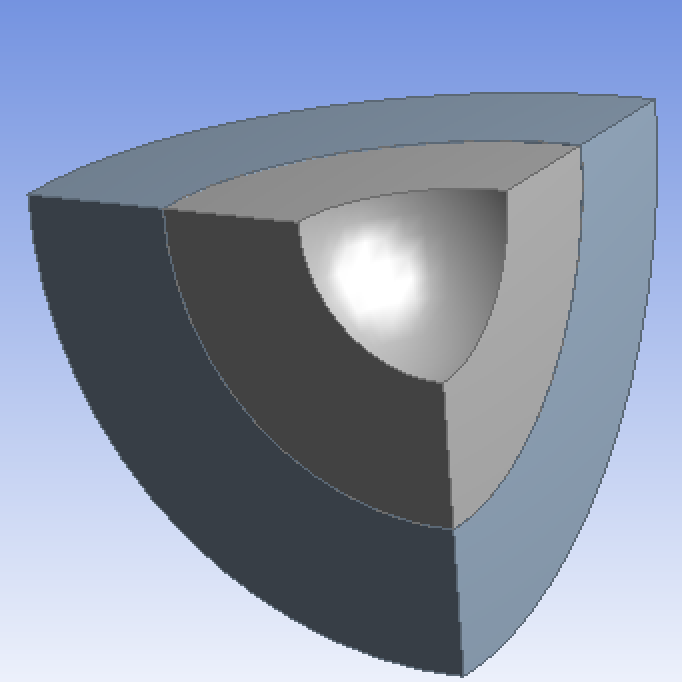
\includegraphics[scale=0.7]{img/Sphere.png} \\
  \caption{Восьмая часть двухслойной полой сферы.}
  \label{fig_1}
\end{figure}
\newpage

\subsection{Математическая постановка задачи}

Обозначим

$u_1=u_r(r,\theta,\varphi)$, $u_2=u_{\theta}(r,\theta,\varphi)$, $u_3=u_{\varphi}(r,\theta,\varphi)$ -- компоненты вектора перемещений;

$\varepsilon_{11}=\varepsilon_{rr}$, $\varepsilon_{22}=\varepsilon_{\theta\theta}$, $\varepsilon_{33}=\varepsilon_{\varphi\varphi}$,
$\varepsilon_{12}=\varepsilon_{21}=\varepsilon_{r\theta}$,
$\varepsilon_{23}=\varepsilon_{32}=\varepsilon_{\theta\varphi}$,
$\varepsilon_{13}=\varepsilon_{31}=\varepsilon_{r\varphi}$ -- компоненты тензора малых деформаций;

$\sigma_{11}=\sigma_{rr}$, $\sigma_{22}=\sigma_{\theta\theta}$, $\sigma_{33}=\sigma_{\varphi\varphi}$,
$\sigma_{12}=\sigma_{21}=\sigma_{r\theta}$,
$\sigma_{23}=\sigma_{32}=\sigma_{\theta\varphi}$,
$\sigma_{13}=\sigma_{31}=\sigma_{r\varphi}$ -- компоненты тензора напряжений.
\newline

Граничные условия:

1) $u_1^{i}|_{r=a}=u_0$ -- нагружение внутренней поверхности внезапно возникшим перемещением;

2) $\sigma_{11}^{i}|_{r=b}=\sigma_{11}^{e}|_{r=b}$ -- первое условие идеального контакта слоёв (равенство нормальных составляющих напряжений);

3) $u_1^{i}|_{r=b}=u_1^{e}|_{r=b}$ -- второе условие идеального контакта слоёв (равенство радиальных перемещений);

4) $\sigma_{11}^{e}|_{r=c}=0$ -- внешняя поверхность свободна.
\newline

При заданных параметрах (модуль Юнга и коэффициент Пуассона) упругих материалов внутренней и внешней частей сферы найти зависимость компонент вектора перемещений и тензора напряжений от $r$, $\theta$, $\varphi$ и построить соответствующие графики.
\newline

Решить задачу аналитически, воспользовавшись соотношениями линейной теории упругости, и численно методом конечных элементов.

\newpage

\Large
\section{Решение поставленной задачи}

\subsection{Аналитическое решение}

\normalsize

Удобно применять сферические координаты. В силу центральной симметрии напряженного и деформированного состояний толстостенной сферы все её точки могут перемещаться только в радиальном направлении. Следовательно, ожидаемые деформированное и напряженное состояния не будут зависеть от переменных $\theta$ и $\varphi$.

Общие выражения для компонентов тензора малых деформаций:
\begin{equation}
    \begin{array}{lll}
        \DS \varepsilon_{11} = \dfrac{d u(r)}{dr}, &\quad \DS \varepsilon_{22} = \dfrac{u(r)}{r}, &\quad \DS \varepsilon_{33} = \dfrac{u(r)}{r}
        \\[3mm]
        \varepsilon_{12} = \varepsilon_{21} = 0, &\quad \DS \varepsilon_{13} = \varepsilon_{31} = 0, &\quad \DS \varepsilon_{23} = \varepsilon_{32} = 0.
    \end{array}
\end{equation}

Относительное изменение объёма (объёмное расширение) имеет вид:

\begin{equation}
    \DS \Theta=\dfrac{d u(r)}{dr}+\dfrac{2u(r)}{r}
\end{equation}

Выражения напряжений из закона Гука:
\begin{equation}\label{sigma_components}
    \begin{array}{l}
        \DS \sigma_{11}=\lambda\Theta+2\mu\varepsilon_{11}=\lambda\left(\dfrac{d u(r)}{dr}+\dfrac{2u(r)}{r}\right)+2\mu\dfrac{d u(r)}{dr},
        \\[3mm]
        \DS \sigma_{22}=\lambda\Theta+2\mu\varepsilon_{22}=\lambda\left(\dfrac{d u(r)}{dr}+\dfrac{2u(r)}{r}\right)+2\mu\dfrac{u(r)}{r},
        \\[3mm]
        \DS \sigma_{33}=\lambda\Theta+2\mu\varepsilon_{33}=\lambda\left(\dfrac{d u(r)}{dr}+\dfrac{2u(r)}{r}\right)+2\mu\dfrac{u(r)}{r},
    \end{array}
\end{equation}

Дифференциальное уравнение равновесия без учёта массовых сил запишется в следующем виде:
\begin{equation}\label{equilibrium_eq}
    \DS \nabla \cdot \Tens{\sigma}=0  \Rightarrow  \frac{d \sigma_{11}}{dr}+\dfrac{2\sigma_{11}-\sigma_{22}-\sigma_{33}}{r}=0.
\end{equation}

Подставляя выражения $\sigma_{11}$, $\sigma_{22}$ и $\sigma_{33}$ из (\ref{sigma_components}) в уравнение равновесия (\ref{equilibrium_eq}), получаем:
\begin{equation}
    \DS \lambda\left(\frac{d^2u(r)}{dr^2}+\dfrac{2\left(\dfrac{d u(r)}{dr}\right)}{r}-\dfrac{2u(r)}{r^2}\right)+2\mu\left(\frac{d^2u(r)}{dr^2}+\dfrac{2\left(\dfrac{d u(r)}{dr}\right)}{r}-\dfrac{2u(r)}{r^2}\right)=0.
\end{equation}

Решения полученного дифференциального уравнения равновесия в перемещениях
\begin{equation}
    \DS\frac{d^2u(r)}{dr^2}+\dfrac{2\left(\dfrac{d u(r)}{dr}\right)}{r}-\dfrac{2u(r)}{r^2}=0
\end{equation}
для внутренней и внешней частей составной сферы запишутся в виде:
\begin{equation}\label{sol}
    \begin{array}{ll}
        \DS u^{i}(r)=C_1r+\dfrac{C_2}{r^2}, &\quad u^{e}(r)=C_3r+\dfrac{C_4}{r^2}.
    \end{array}
\end{equation}
Подставим найденные решения (\ref{sol}) в выражение для $\sigma_{11}$ из (\ref{sigma_components}):
\begin{equation}\label{sigma_sol}
    \begin{array}{ll}
        \DS \sigma_{11}^{i}=3\lambda^{i} C_1+2\mu^{i}\left(C_1-\dfrac{2C_2}{r^3}\right), &\quad \sigma_{11}^{e}=3\lambda^{e} C_3+2\mu^{e}\left(C_3-\dfrac{2C_4}{r^3}\right).
    \end{array}
\end{equation}
Подставим полученные выражения (\ref{sol}) и (\ref{sigma_sol}) в граничные условия:
\begin{equation}
\begin{cases}
    \begin{array}{l}
        \DS u^{i}(a)=C_1a+\dfrac{C_2}{a^2}=u_0,
        \\[3mm]
        \DS \sigma_{11}^{i}(b)=\sigma_{11}^{e}(b)\Leftrightarrow 3\lambda^{i} C_1+2\mu^{i}\left(C_1-\dfrac{2C_2}{b^3}\right)=3\lambda^{e} C_3+2\mu^{e}\left(C_3-\dfrac{2C_4}{b^3}\right),
        \\[3mm]
        \DS u^{i}(b)=u^{e}(b)\Leftrightarrow C_1r+\dfrac{C_2}{b^2}=C_3r+\dfrac{C_4}{b^2},
        \\[3mm]
        \DS \sigma_{11}^{e}(c)=3\lambda^{e} C_3+2\mu^{e}\left(C_3-\dfrac{2C_4}{c^3}\right)=0.
    \end{array}
\end{cases}
\end{equation}

Решая полученную систему четырёх алгебраических уравнений с четырьмя неизвестными в системе символьных вычислений Maple, находим постоянные интегрирования:
\begin{figure}[H]
  \centering
  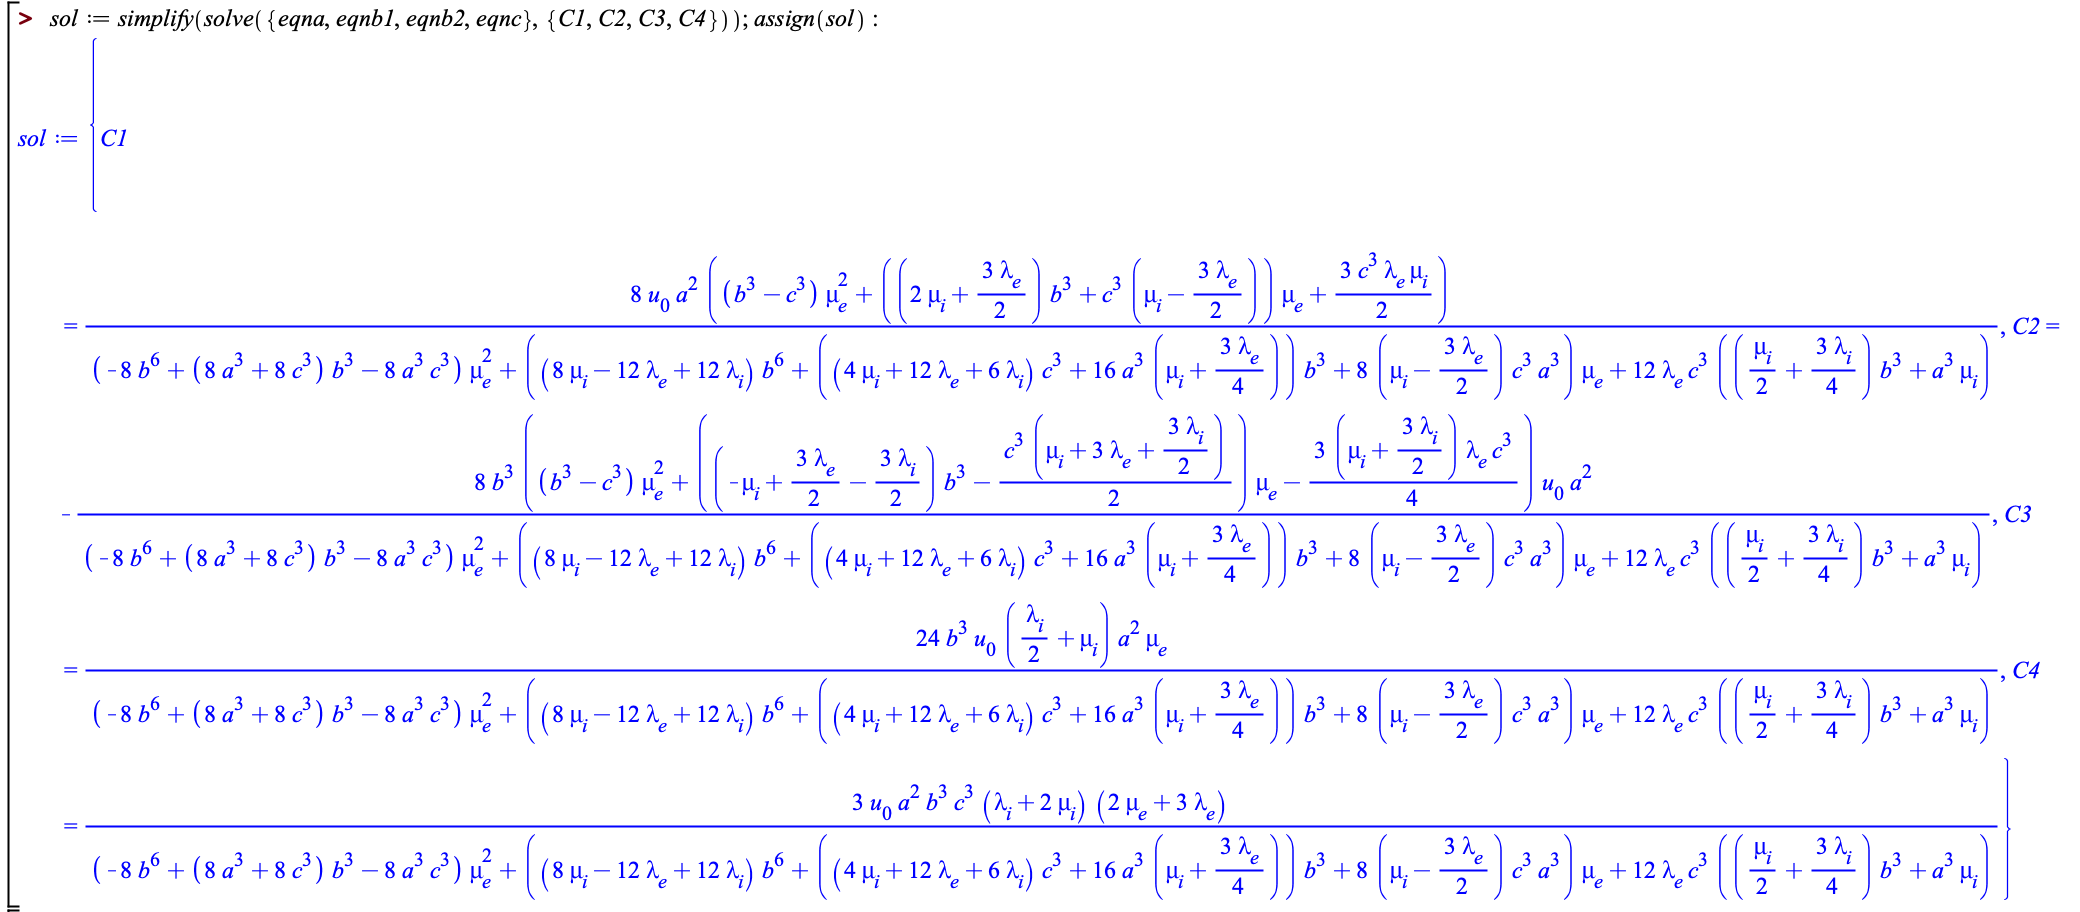
\includegraphics[scale=0.47]{img/IntConst_Lab1.png}\\
  \caption{Постоянные интегрирования.}
  \label{fig_2}
\end{figure}


Подставляя найденные константы в (\ref{sigma_sol}), находим $\sigma_{11}^{i}$ и $\sigma_{11}^{e}$:
\begin{figure}[H]
  \centering
  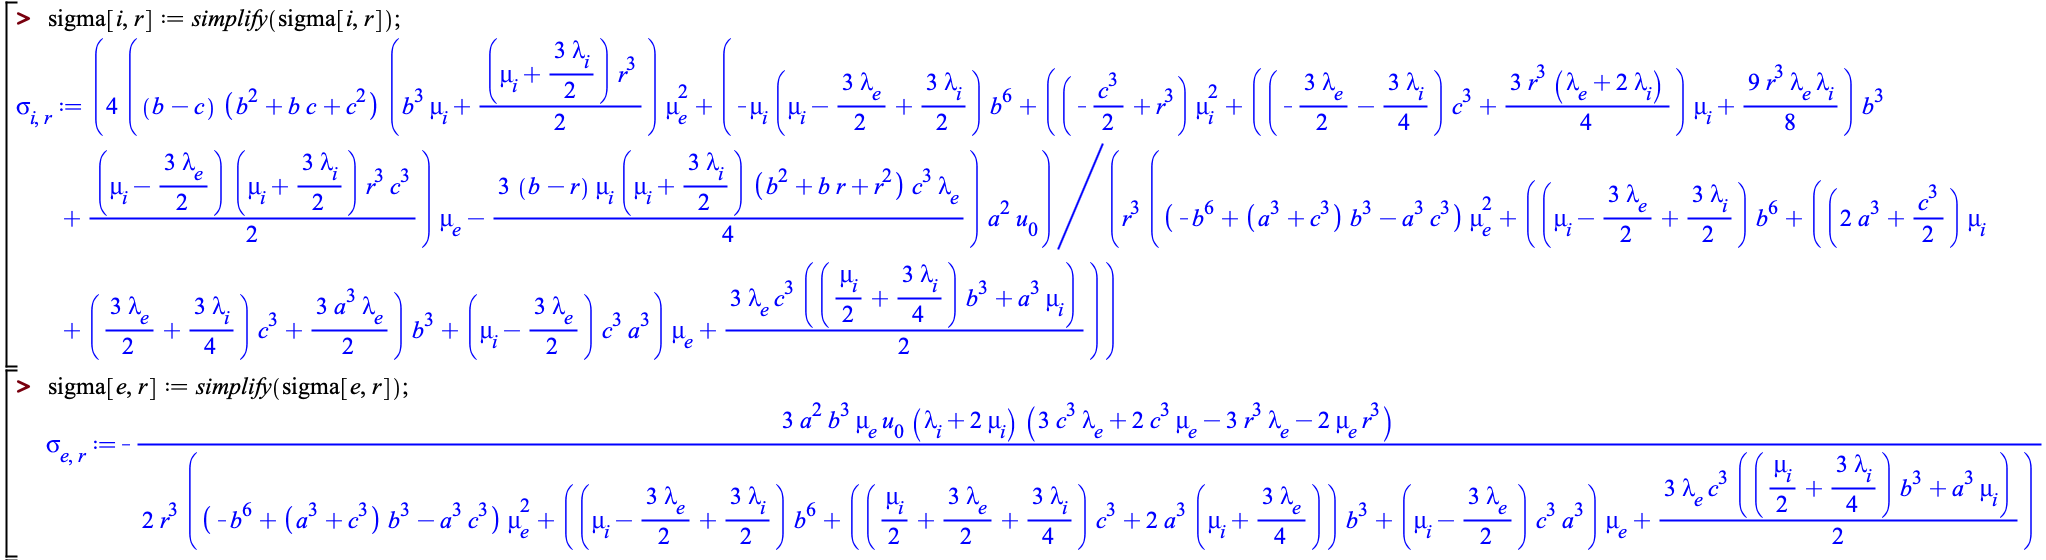
\includegraphics[scale=0.45]{img/Sigma11_Lab1.png}\\
  \caption{Компонента $\sigma_{11}$ тензоров напряжений для внутренней и внешней частей сферы.}
  \label{fig_3}
\end{figure}

Аналогично находим оставшиеся диагональные компоненты тензоров напряжений и радиальные перемещения точек внутренней и внешней частей составной сферы:

\begin{figure}[H]
  \centering
  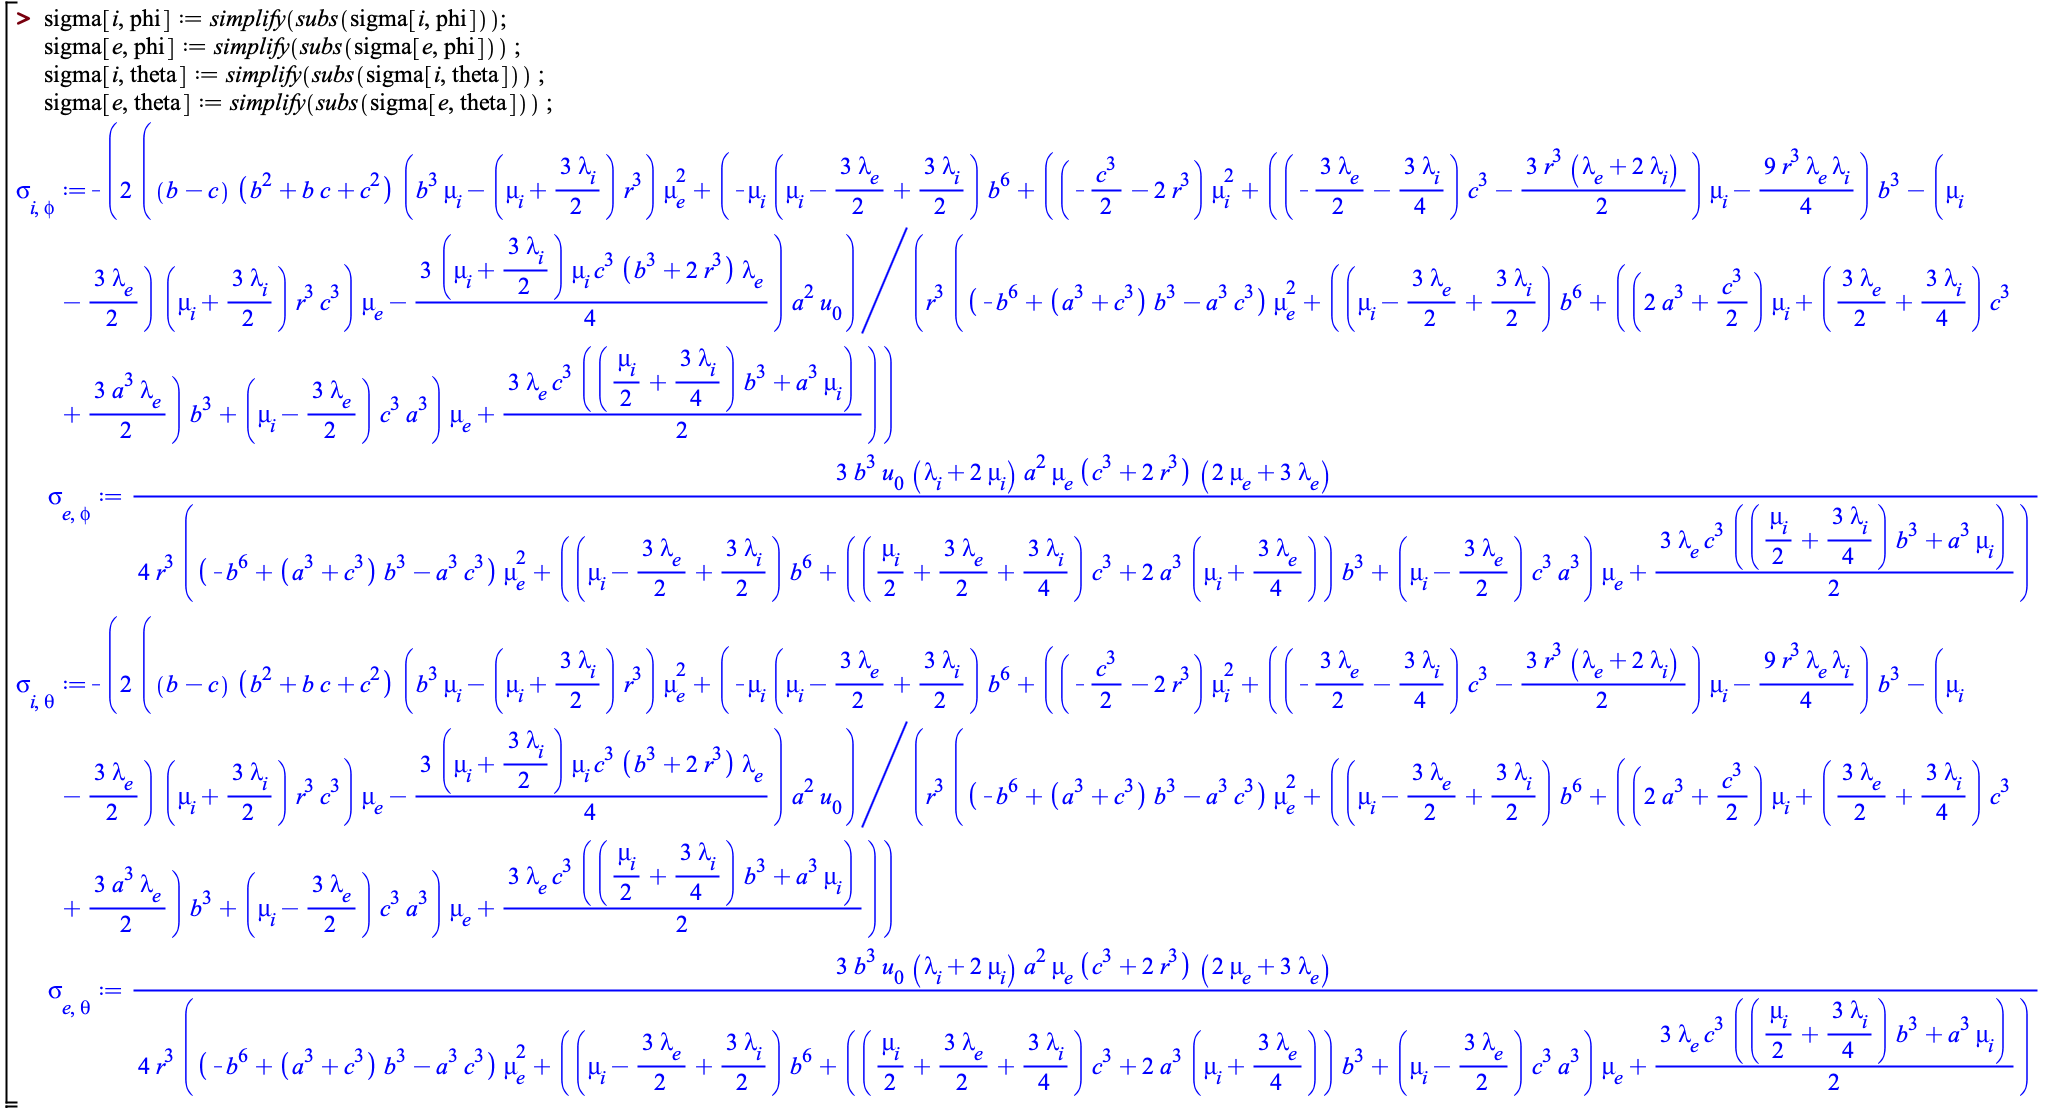
\includegraphics[scale=0.47]{img/Sigma_theta_Lab1.png}\\
  \caption{Компоненты $\sigma_{22}$ и $\sigma_{33}$ тензоров напряжений для внутренней и внешней частей сферы.}
  \label{fig_4}
\end{figure}

\begin{figure}[H]
  \centering
  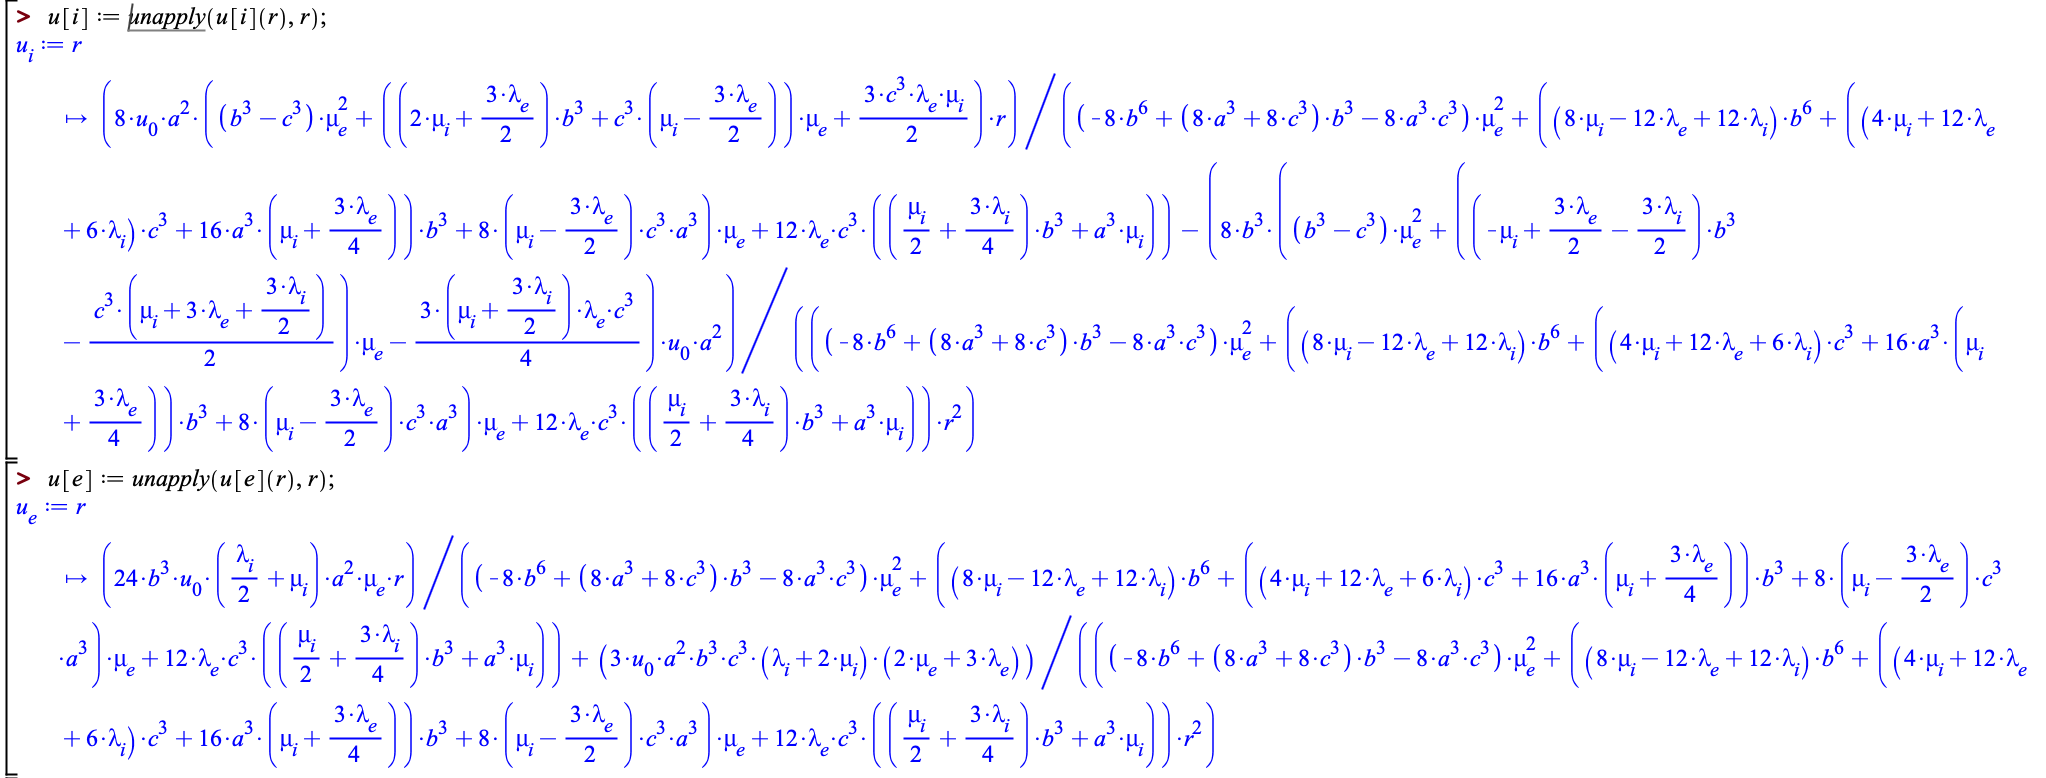
\includegraphics[scale=0.47]{img/Displacement_Lab1.png}\\
  \caption{Радиальные перемещения точек внутренней и внешней частей сферы.}
  \label{fig_5}
\end{figure}
\newpage
Зададим конкретные значения параметров задачи (Рис. 6). В аналитическом решении все численные значения задаём в СИ. Модуль Юнга и коэффициент Пуассона внутренней части сферы, выполненной из стали, равны соответственно $E^{i}=2.1\cdot 10^{11}$ Па и $\nu^{i}=0.3$, а модуль Юнга и коэффициент Пуассона внешней части сферы, выполненной из меди, $E^{e}=1.3\cdot 10^{11}$ Па и $\nu^{e}=0.34$.

\begin{figure}[H]
  \centering
  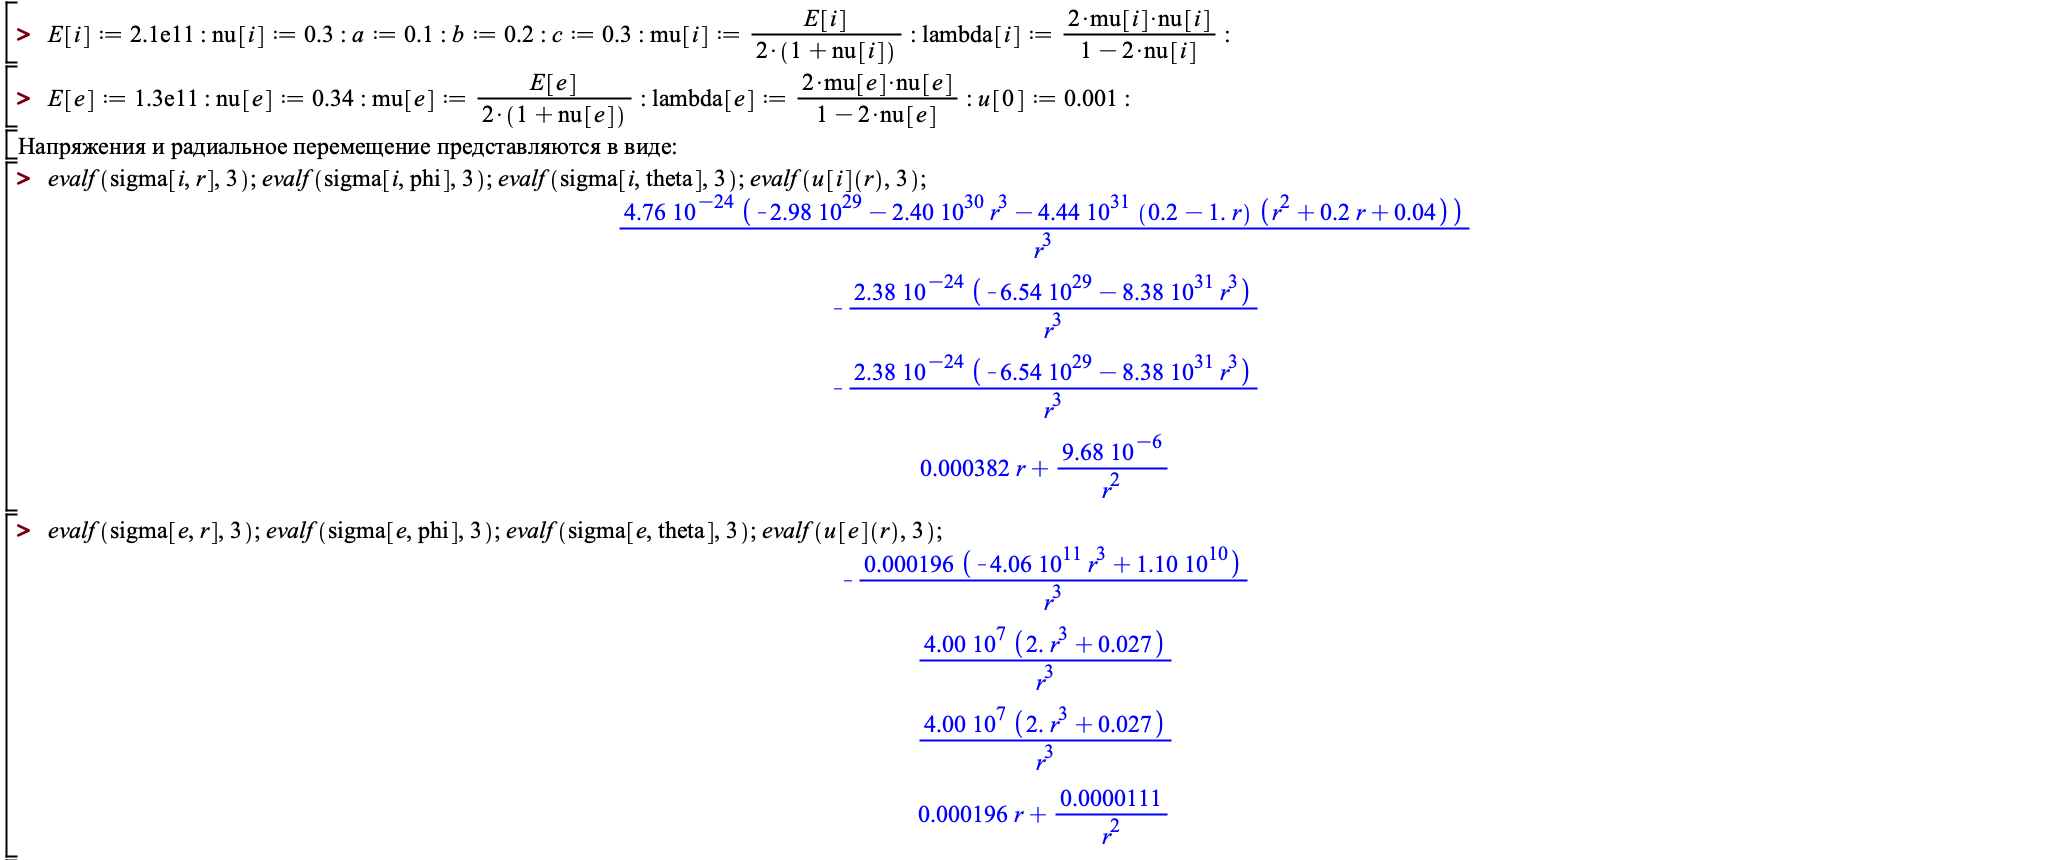
\includegraphics[scale=0.55]{img/Parameters_Lab1.png}\\
  \caption{Числовые значения параметров задачи.}
  \label{fig_6}
\end{figure}
Построим графики зависимости радиальных, тангенциальных напряжений и радиальных перемещений от $r$ (Рис. 7, Рис. 8 и Рис. 9):

\begin{figure}[H]
    \centering
    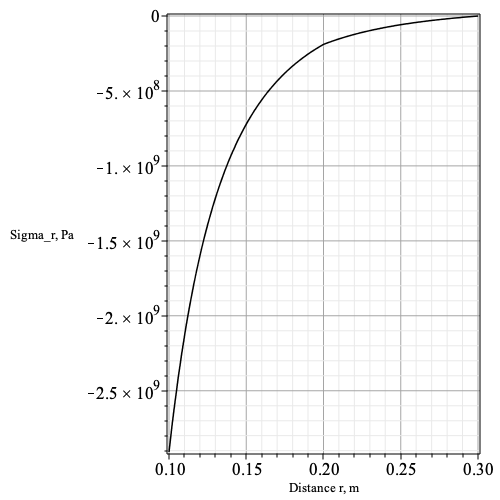
\includegraphics[scale=0.6]{img/Graph1_Lab1.png}\\
    \caption{График зависимости $\sigma_{11}$ от $r$.}
    \label{fig_7}
\end{figure}

    
\begin{figure}[H]
    \centering
    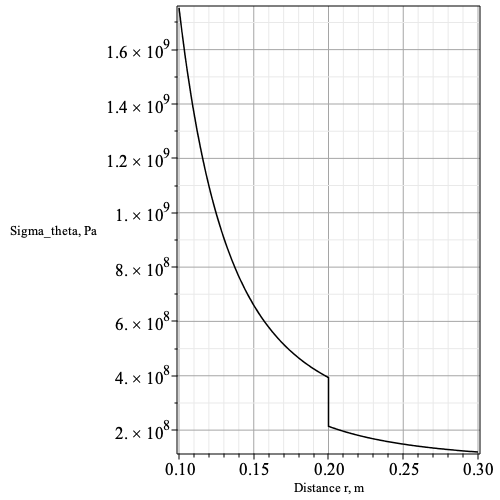
\includegraphics[scale=0.6]{img/Graph3_Lab1.png}\\
    \caption{График зависимости $\sigma_{22}$ от $r$.}
    \label{fig_8}
\end{figure}



\begin{figure}[H]
  \centering
  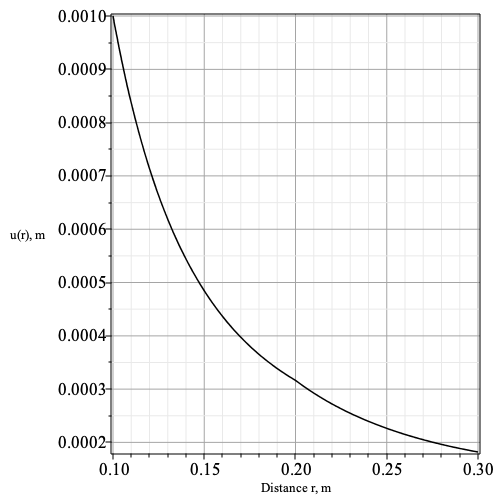
\includegraphics[scale=0.68]{img/Graph4_Lab1.png}\\
  \caption{График зависимости радиальных перемещений от $r$.}
  \label{fig_9}
\end{figure}
Видим, что графики зависимостей радиальных напряжений $\sigma_{11}(r)$ и радиальных премещений $u(r)$ состыкуются на границе слоёв (условия идеального контакта слоёв выполнены), однако испытывают разрыв первой производной. Графики зависимостей тангенциальных напряжений $\sigma_{22}(r)$ и $\sigma_{33}(r)$ испытывают разрыв на границе слоёв, так как параметры (коэффициенты Ламе) внутреннего и внешнего материалов разные.
\newpage

\subsection{Решение в конечно-элементном пакете ANSYS}

В КЭМ-пакете рассматривается одна восьмая составной полой сферы (Рис. 1). Расчёты производятся для одной восьмой части сферы, чтобы существенно сократить количество конечных элементов и время расчёта. Сетка представлена на Рис. 10.

Внутренний слой (модуль Юнга $E=2.1\cdot10^{11}$ Па, коэффициент Пуассона $\nu=0.3$) и внешний слой (модуль Юнга $E=1.3\cdot10^{11}$ Па, коэффициент Пуассона $\nu=0.34$) составной сферы выполнены из упругих материалов.

Внутренняя поверхность нагружается перемещением 1 мм в радиальном направлении, т.е. по нормали к поверхности (Рис. 11).

Для того, чтобы перемещения были только по радиусу, для каждой из трёх граней одной восьмой части сферы задаётся нулевое перемещение вдоль оси, перпендикулярной к этой грани. В частности, для грани, лежащей в плоскости xOz, задали нулевое перемещение по оси Oy (Рис. 12).

\begin{figure}[H]
  \centering
  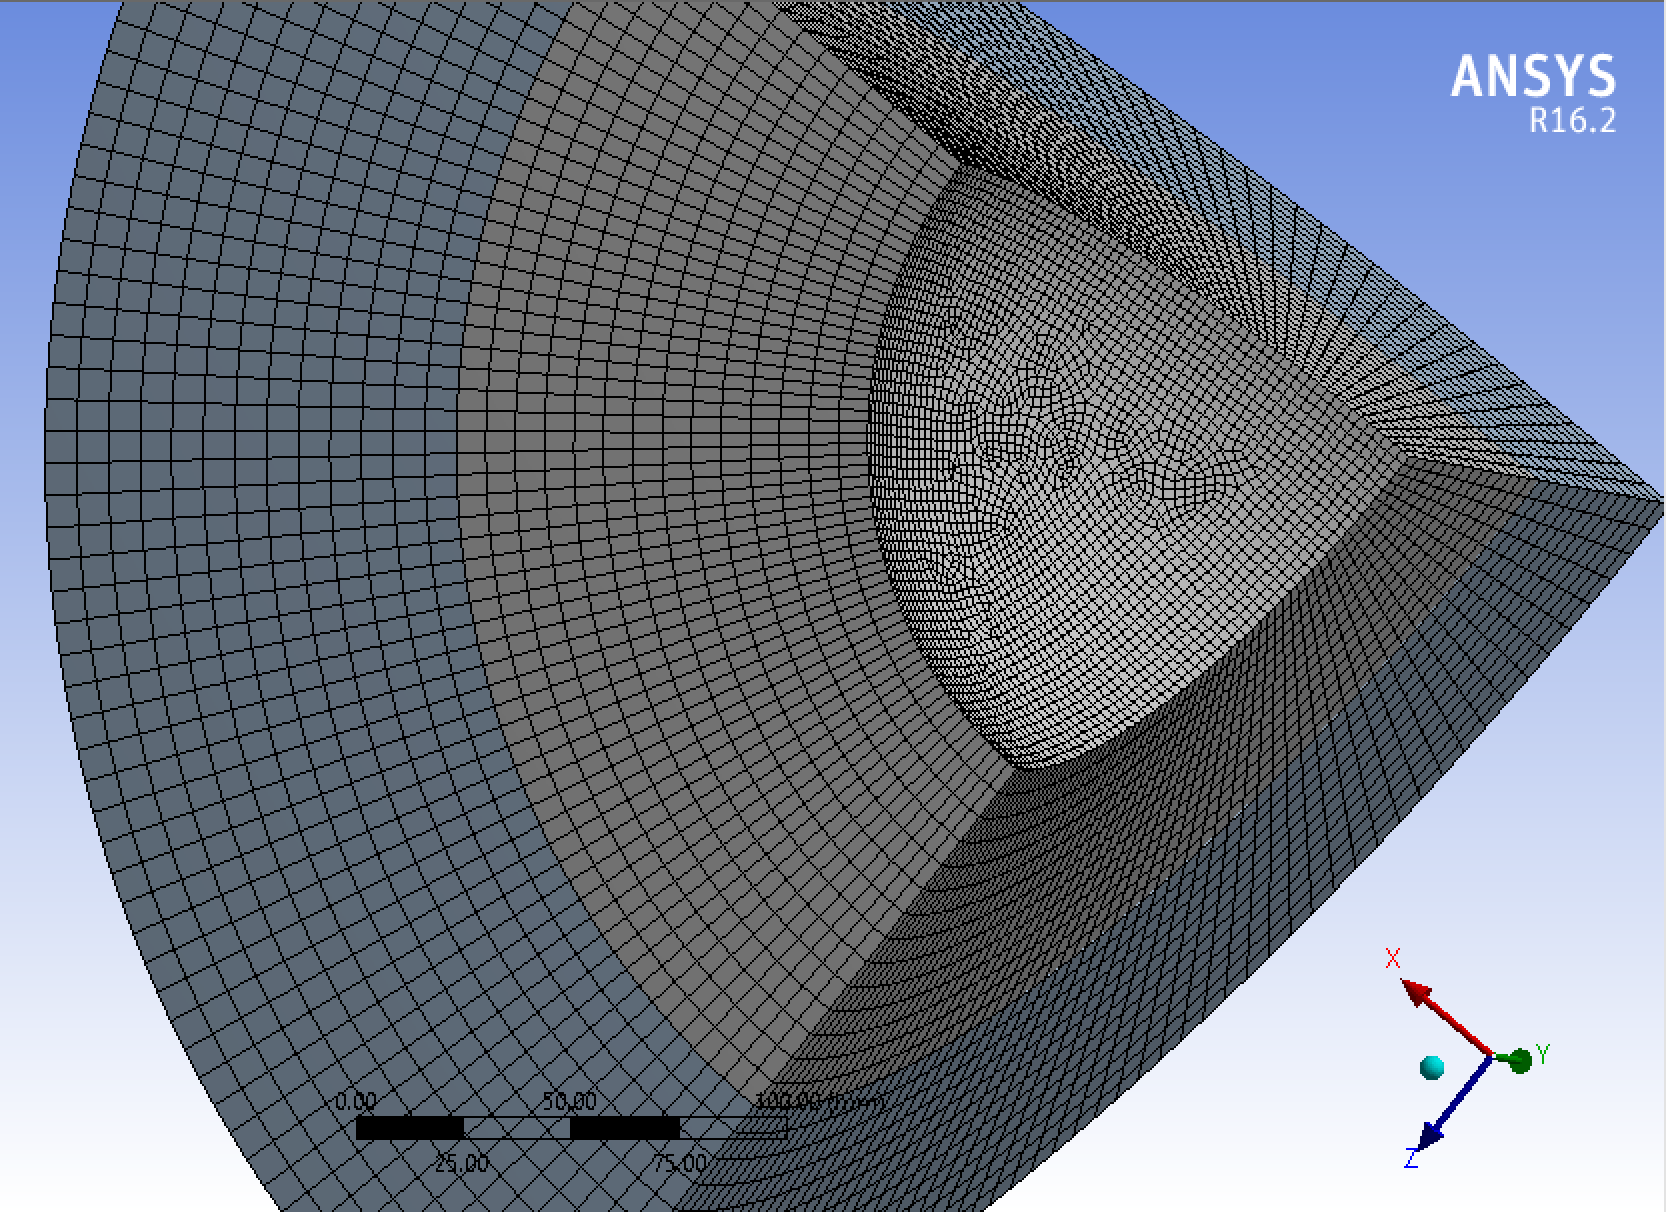
\includegraphics[scale=0.45]{img/Mesh.png}\\
  \caption{Сетка.}
  \label{fig_10}
\end{figure}

\begin{figure}[H]
  \centering
  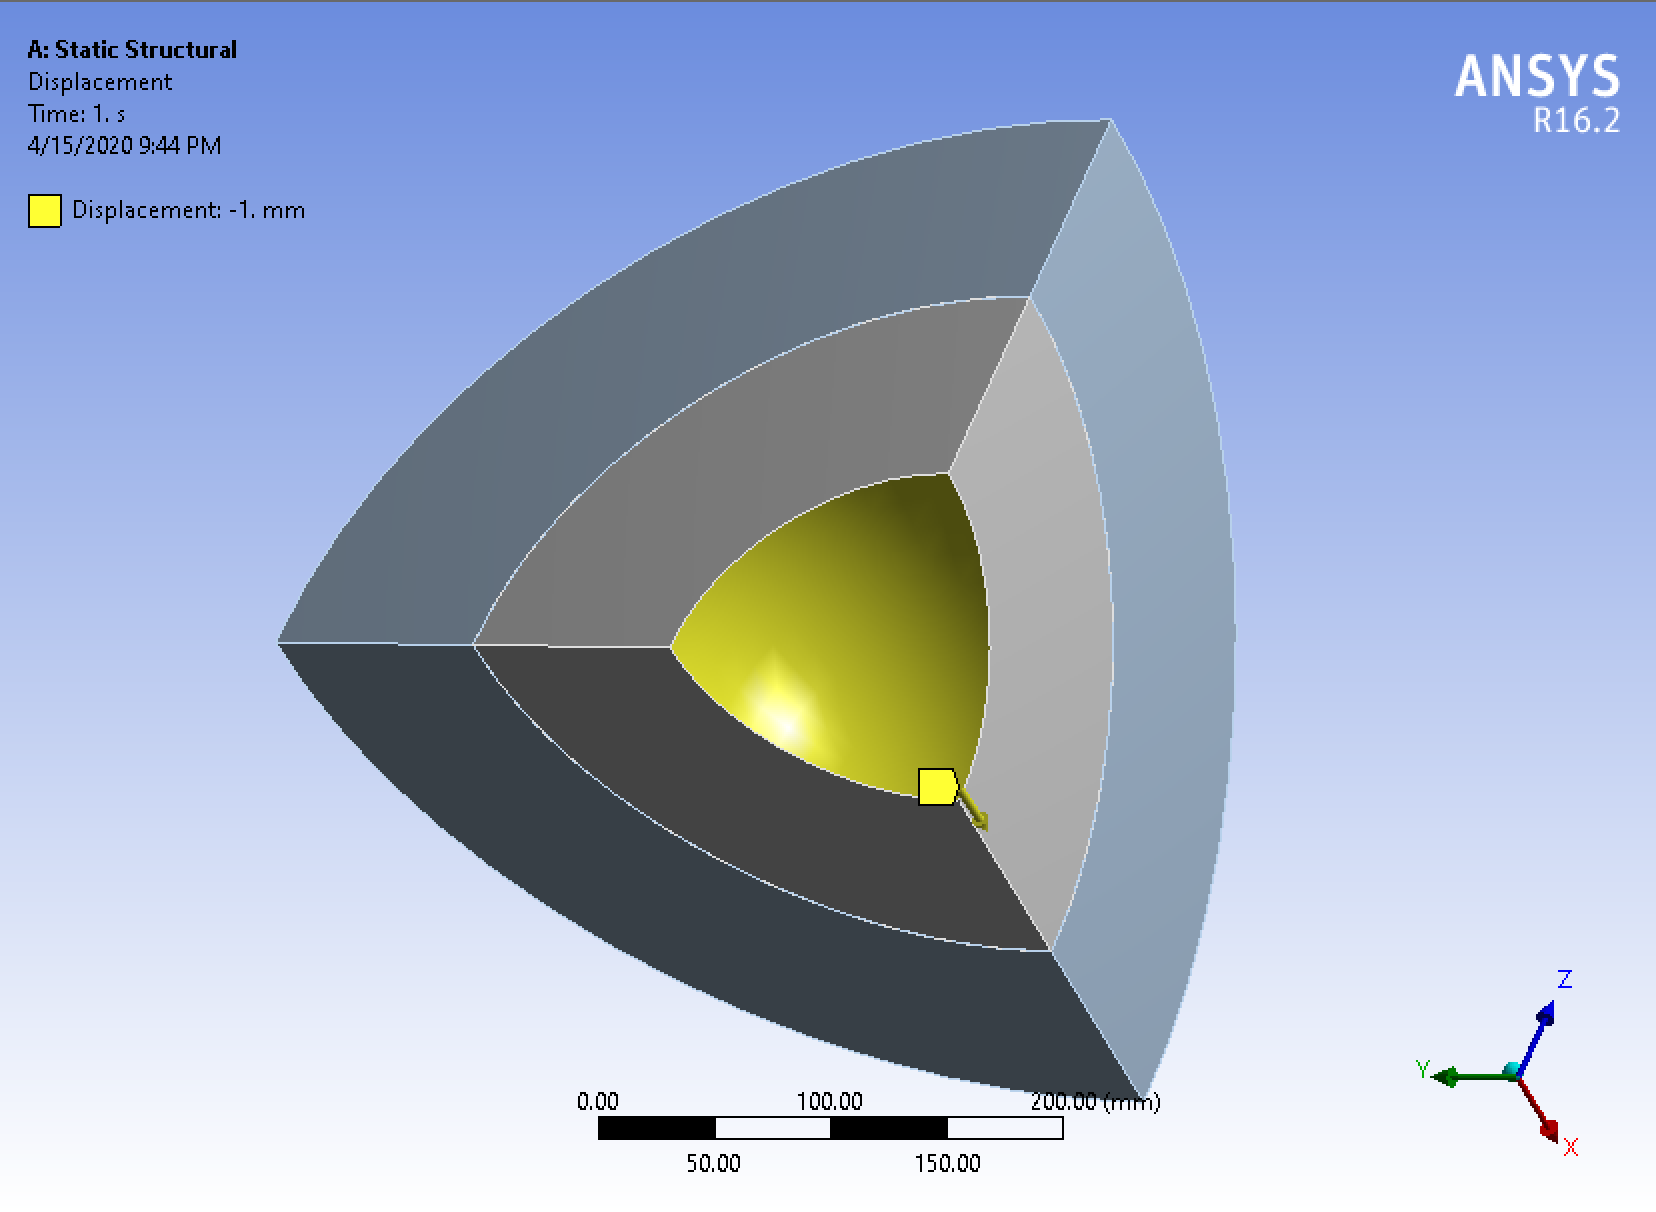
\includegraphics[scale=0.5]{img/Displacement.png}\\
  \caption{Граничное условие на внутреннюю поверхность.}
  \label{fig_11}
\end{figure}

\begin{figure}[H]
  \centering
  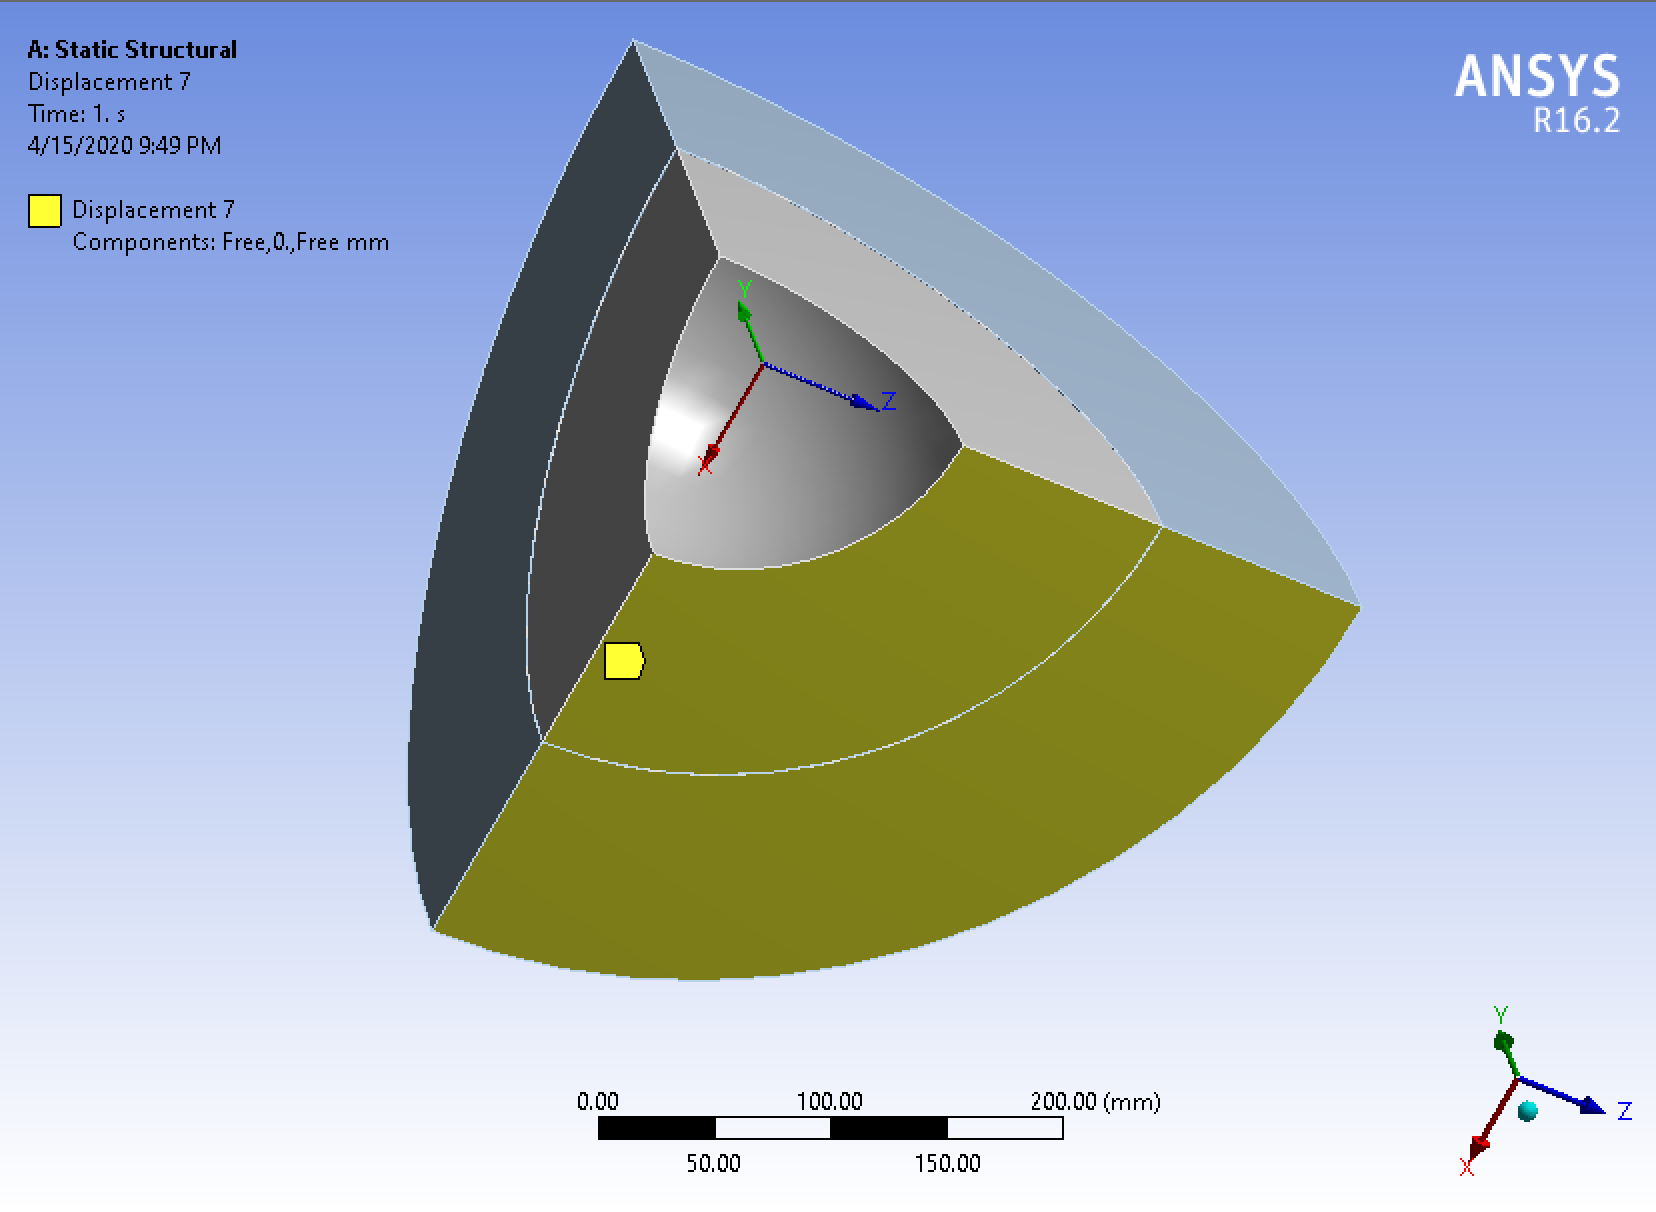
\includegraphics[scale=0.5]{img/Boundary.png}\\
  \caption{Граничное условие на грань (две другие грани - аналогично).}
  \label{fig_12}
\end{figure}

\begin{figure}[H]
  \centering
  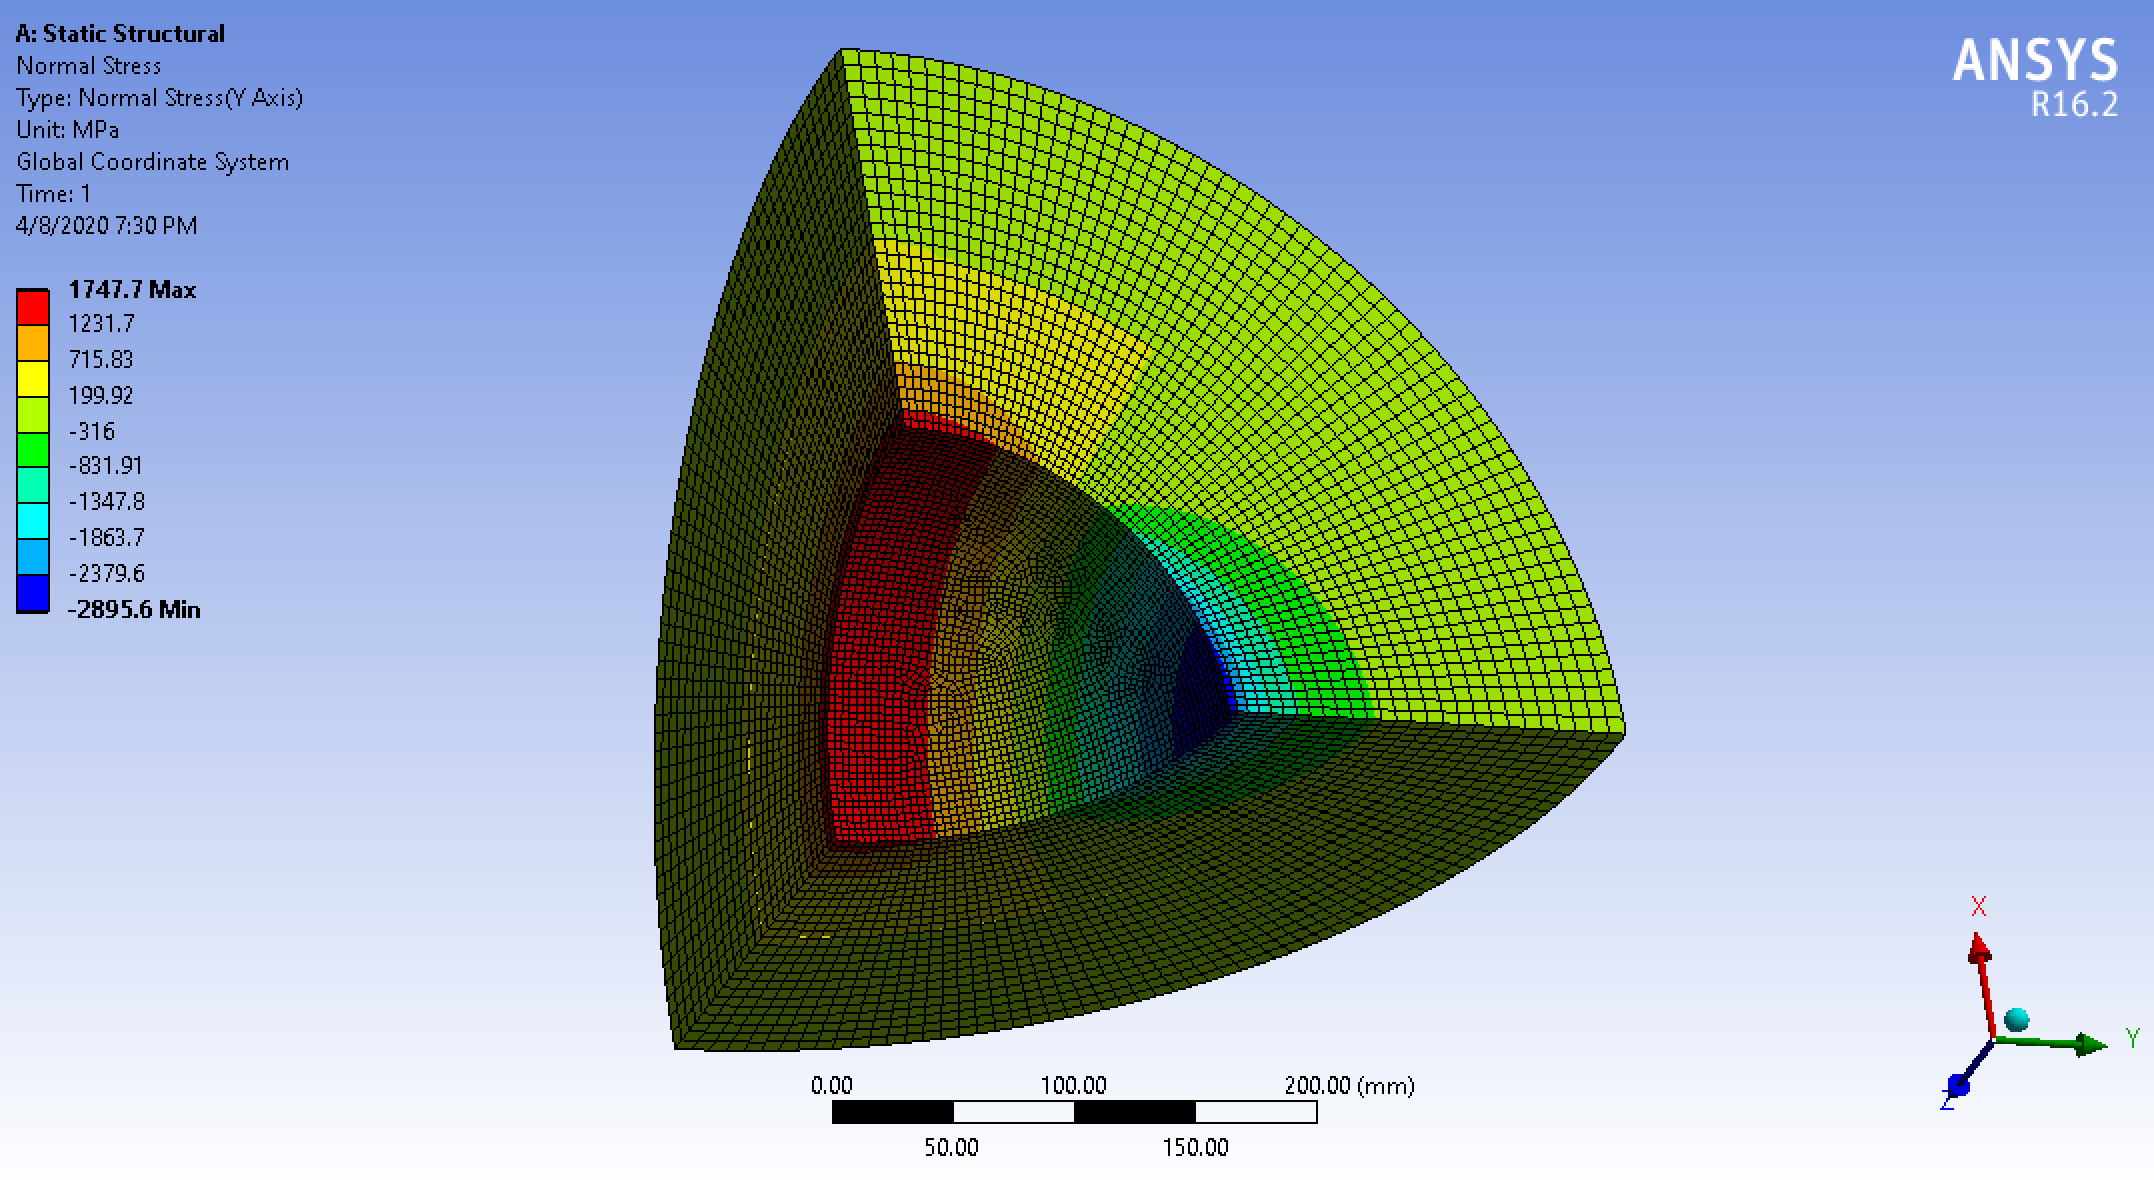
\includegraphics[scale=0.45]{img/Results_NS_Y_Axis.png}\\
  \caption{Распределение напряжений, направленных вдоль оси Oy.}
  \label{fig_13}
\end{figure}

На Рис. 13 построено распределение напряжений, направленных вдоль оси Oy. Следовательно, значения вдоль радиуса по ребру, лежащему на оси Oy, представляют собой радиальные напряжения $\sigma_{11}$, а значения вдоль радиуса по ребру, лежащему на оси Ox, есть тангенциальные напряжения $\sigma_{22}$ и $\sigma_{33}$. Соответственно, на Рис. 13 синим цветом обозначено максимальное (по модулю) радиальное напряжение, а красным цветом -- максимальные (по модулю) тангенциальные напряжения. Значения этих напряжений из colorbar $\mathrm{max}(\left|\sigma_{11}(r)\right|)\approx2.9\cdot10^{9}$ Па и $\mathrm{max}(\left|\sigma_{22}(r)\right|)=\mathrm{max}(\left|\sigma_{33}(r)\right|)\approx1.75\cdot10^{9}$ Па совпадают (с относительной погрешностью, не превышающей $6\%$) со значениями, полученными аналитически (Рис. 7 и Рис. 8).

\begin{figure}[H]
  \centering
  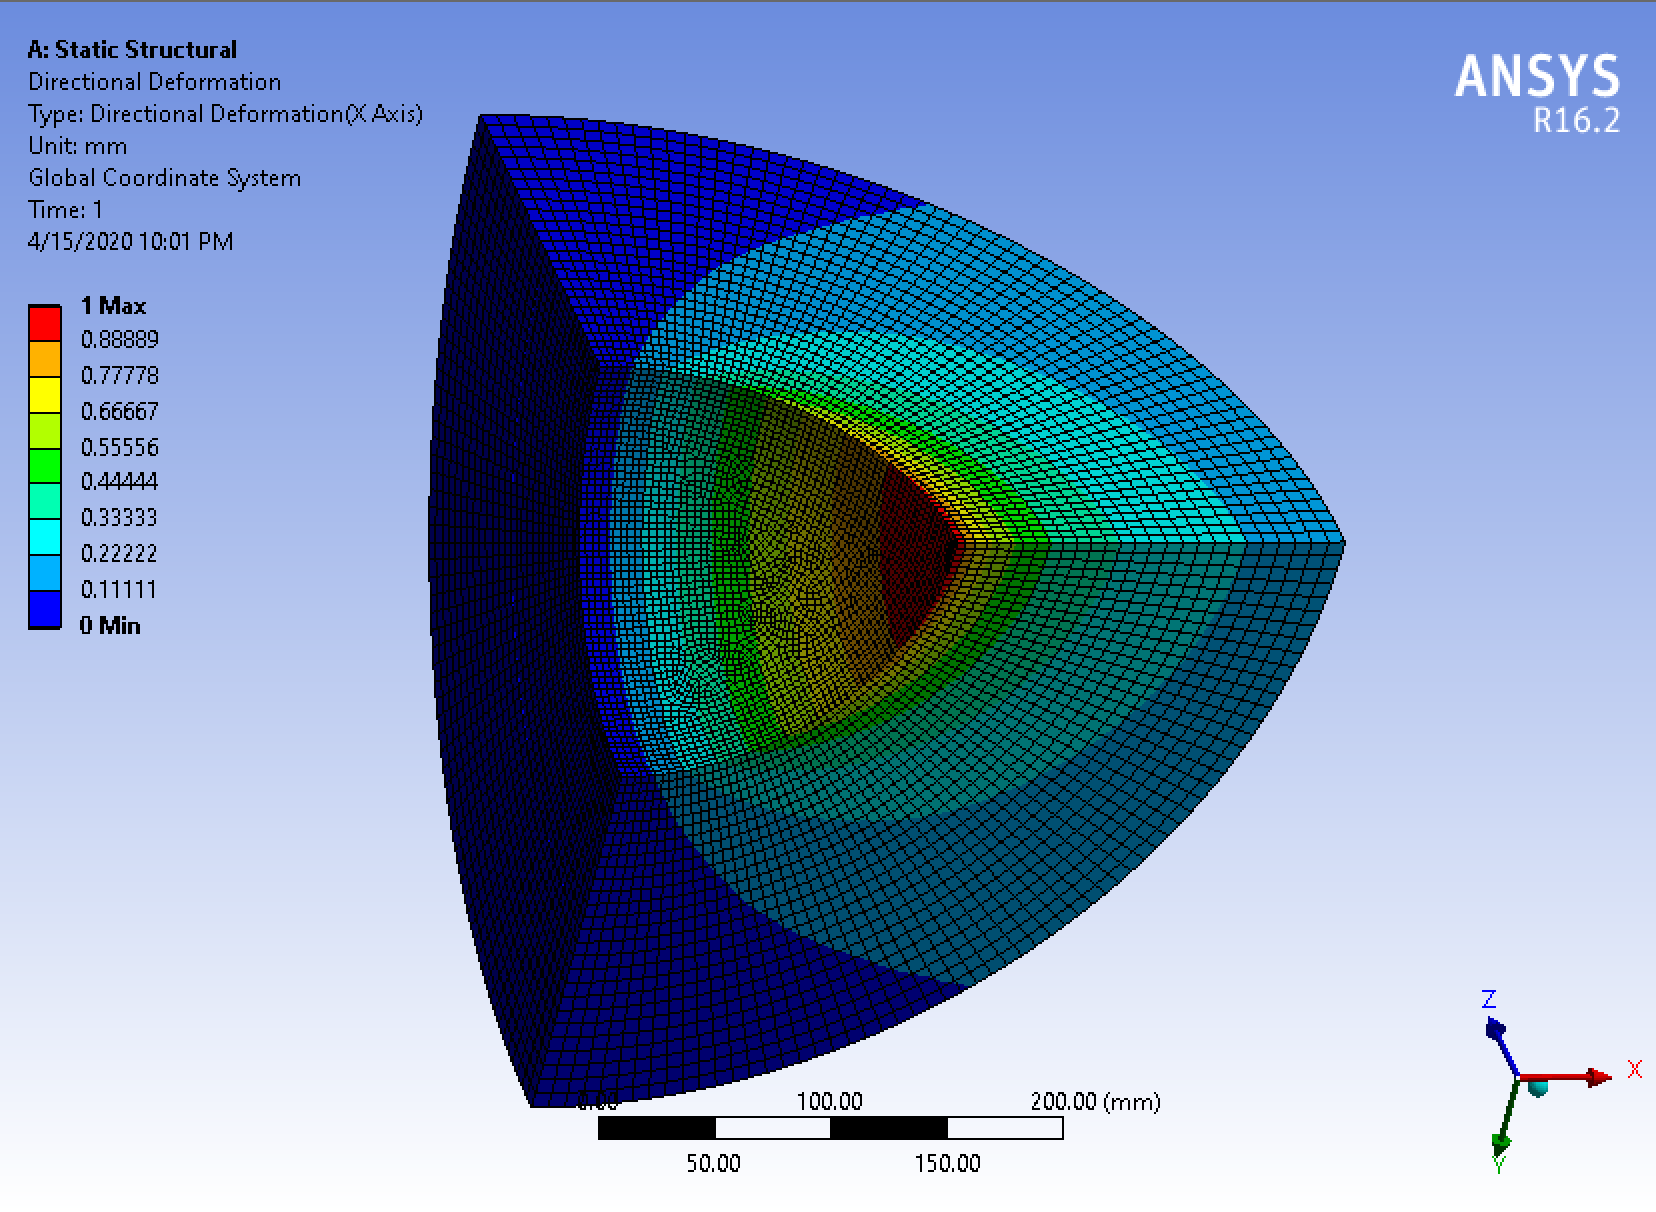
\includegraphics[scale=0.45]{img/Results_Deform_X_Axis.png}\\
  \caption{Распределение деформаций, направленных вдоль оси Ox.}
  \label{fig_14}
\end{figure}
На Рис. 14 построено распределение перемещений, направленных вдоль оси Ox. Следовательно, значения вдоль радиуса по ребру, лежащему на оси Ox, представляют собой радиальные перемещения $u(r)$. Видим, что максимальное радиальное перемещение равно 1 мм (граничное условие выполнено). Также на Рис. 14 отображено отсутствие тангенциальных перемещений.

В MS Excel построим графики зависимостей $\sigma_{11}(r)$, $\sigma_{22}(r)$ и $u(r)$. Значения функций получены в ANSYS.

\begin{figure}[H]
  \centering
  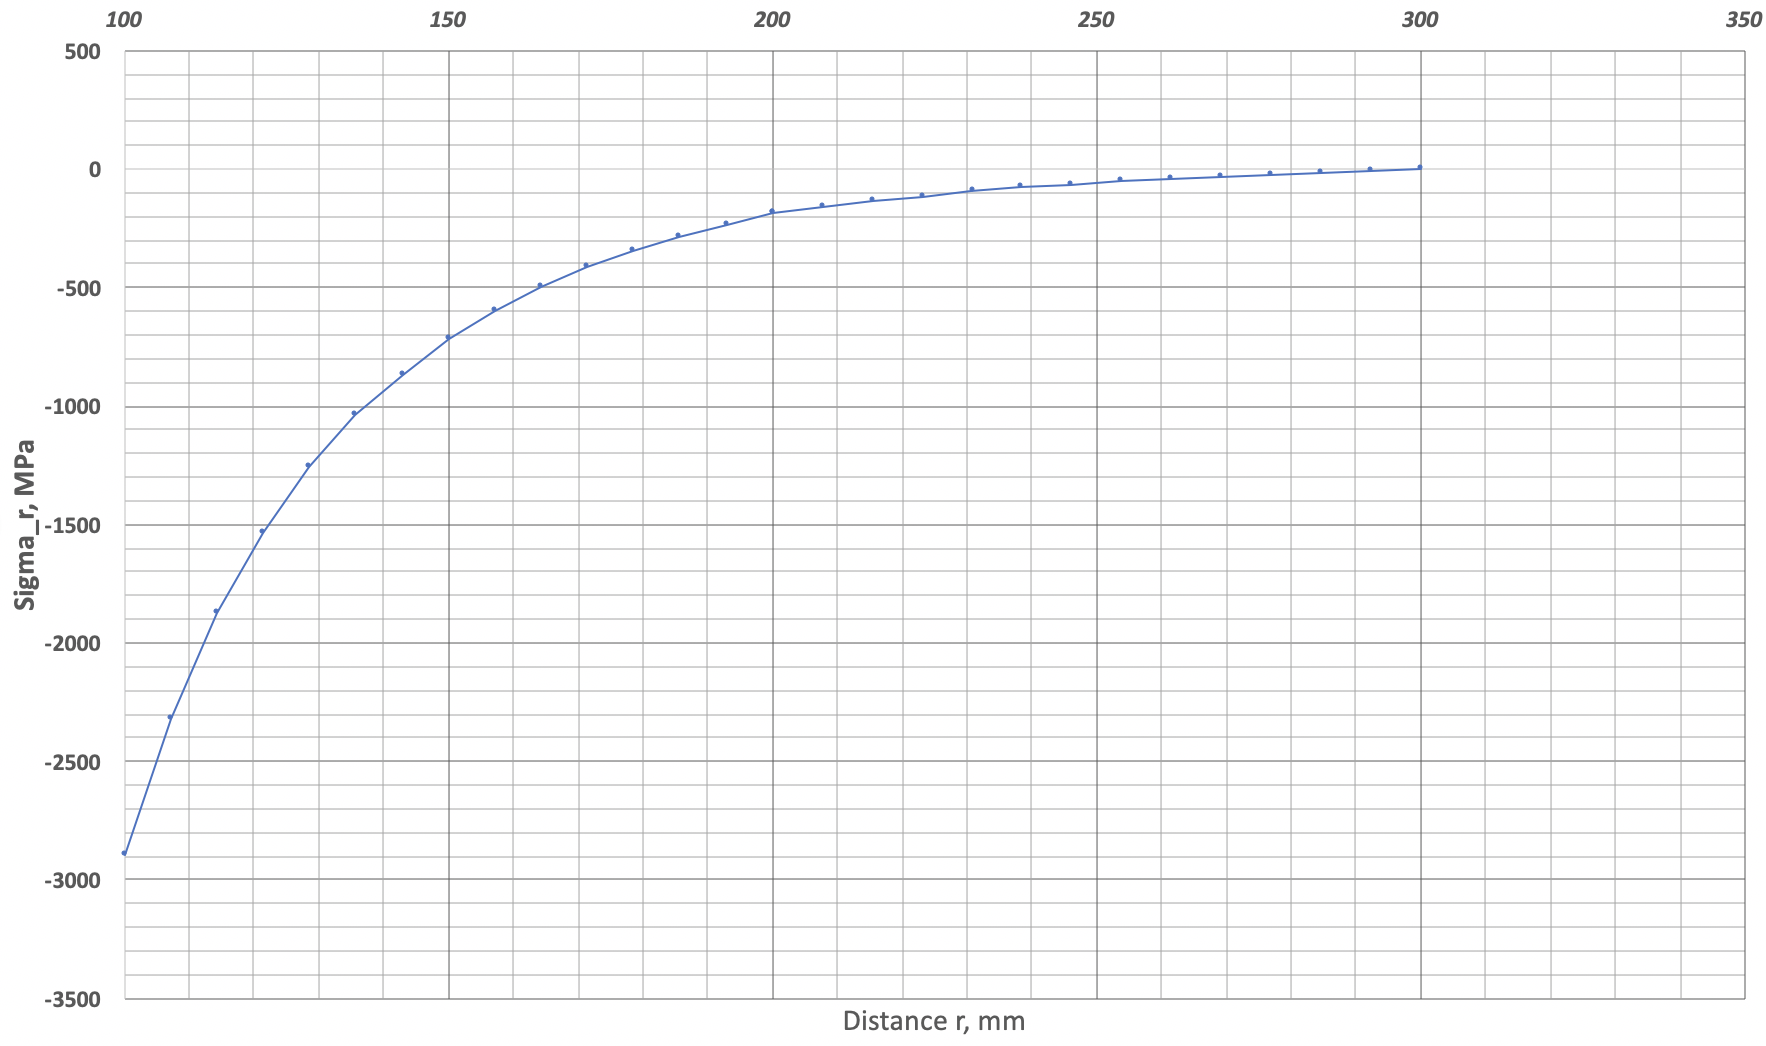
\includegraphics[scale=0.5]{img/Sigma_r_2.png}\\
  \caption{Зависимость радиальных напряжений от радиуса.}
  \label{fig_15}
\end{figure}

\begin{figure}[H]
  \centering
  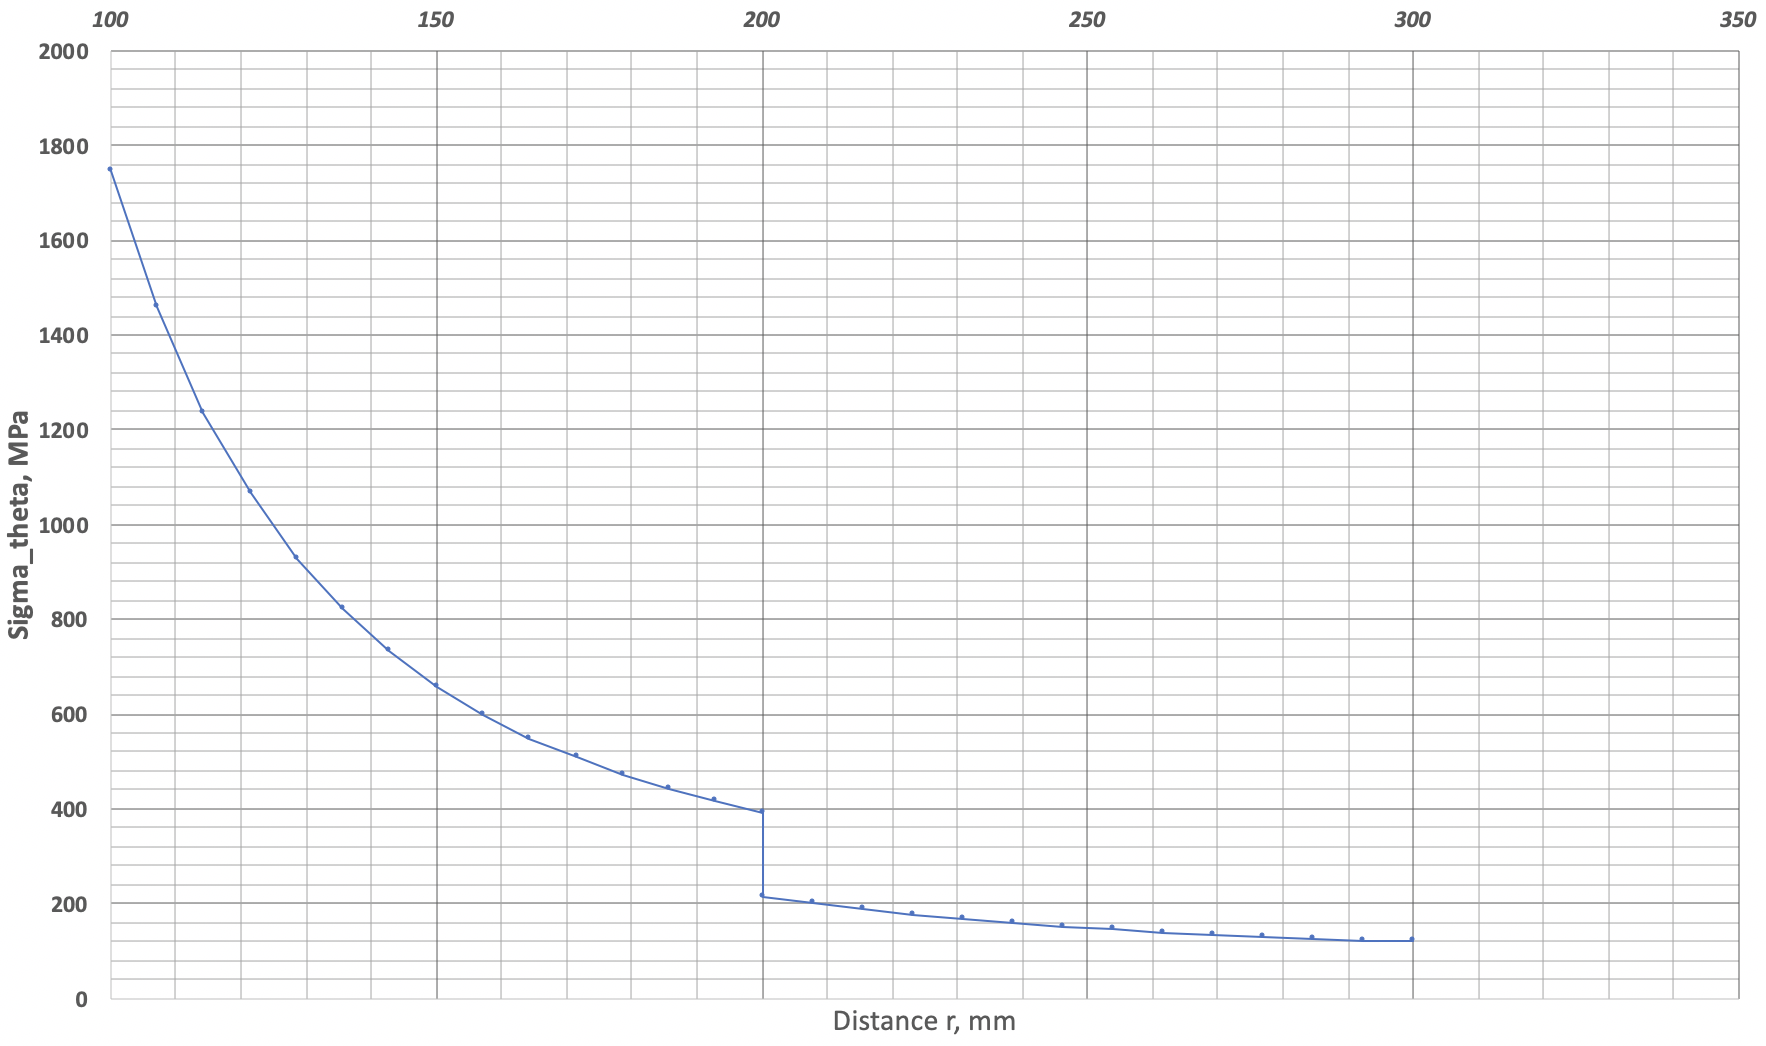
\includegraphics[scale=0.5]{img/Sigma_theta_2.png}\\
  \caption{Зависимость тангенциальных напряжений от радиуса.}
  \label{fig_16}
\end{figure}

\begin{figure}[H]
  \centering
  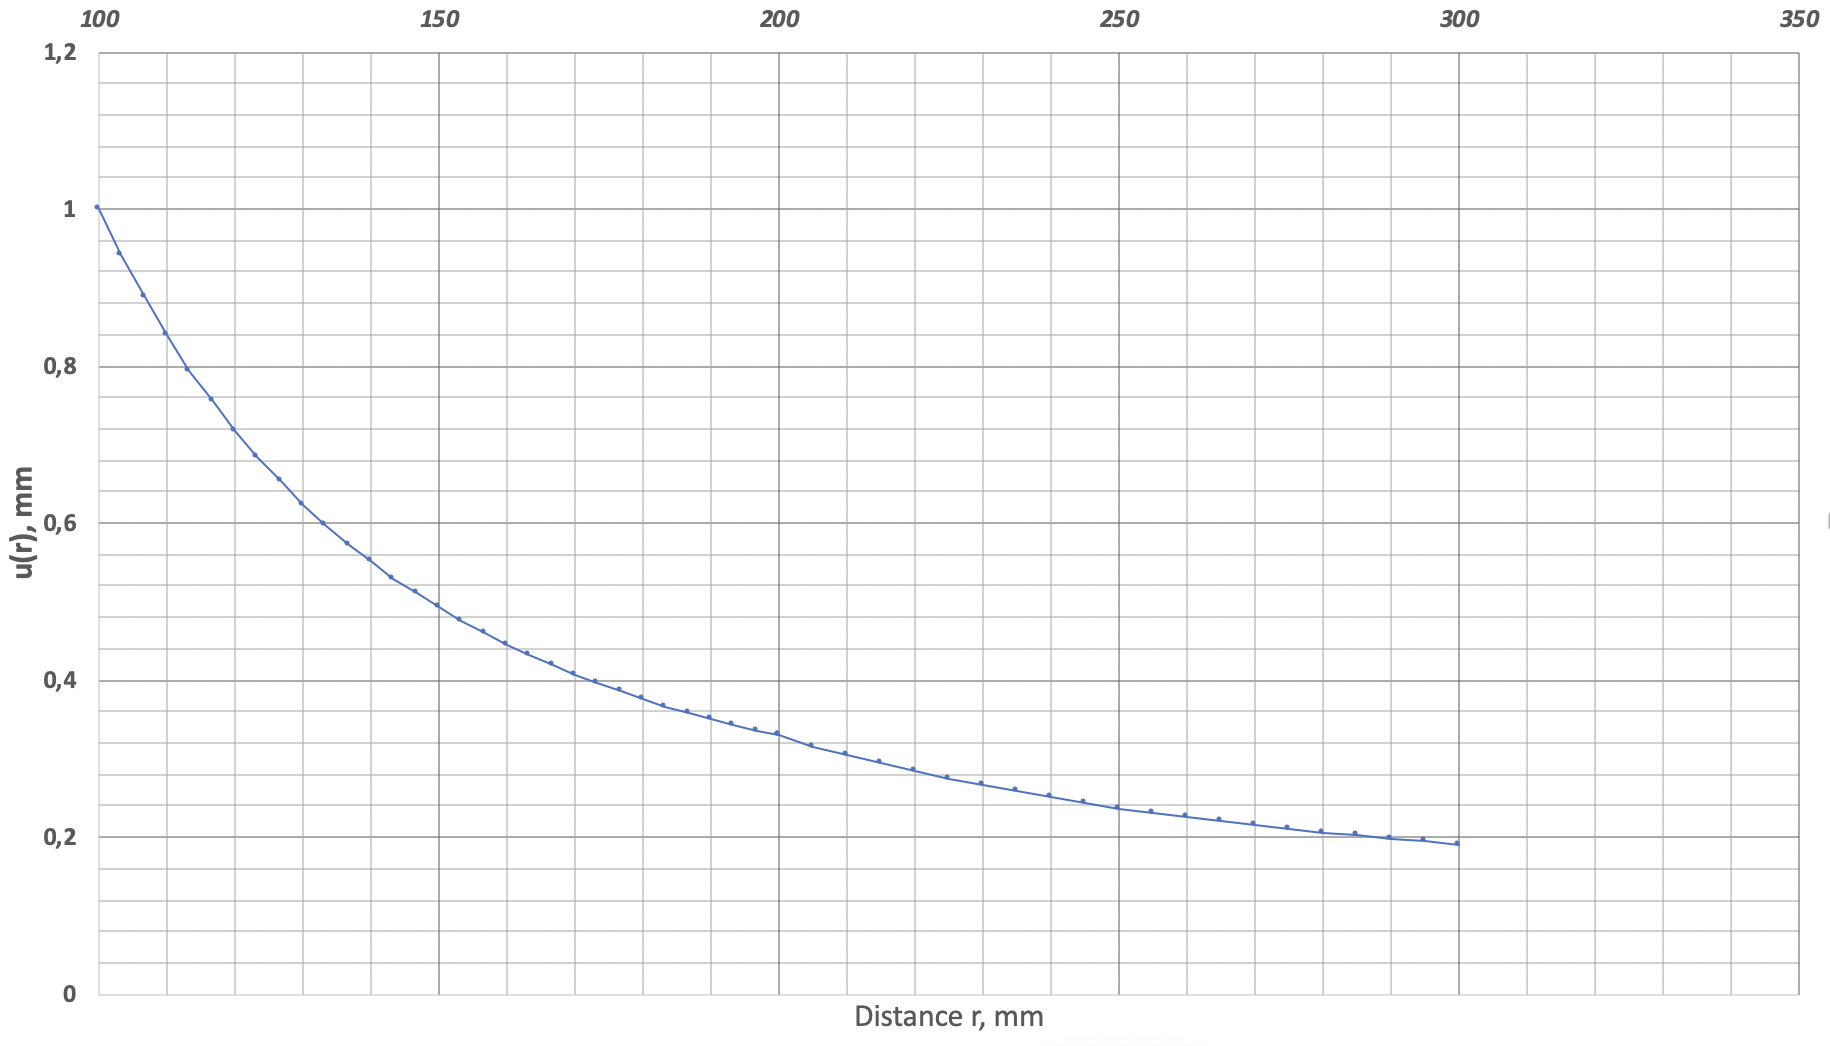
\includegraphics[scale=0.5]{img/u_r.png}\\
  \caption{Зависимость радиальных перемещений от радиуса.}
  \label{fig_17}
\end{figure}

\begin{figure}[H]
  \centering
  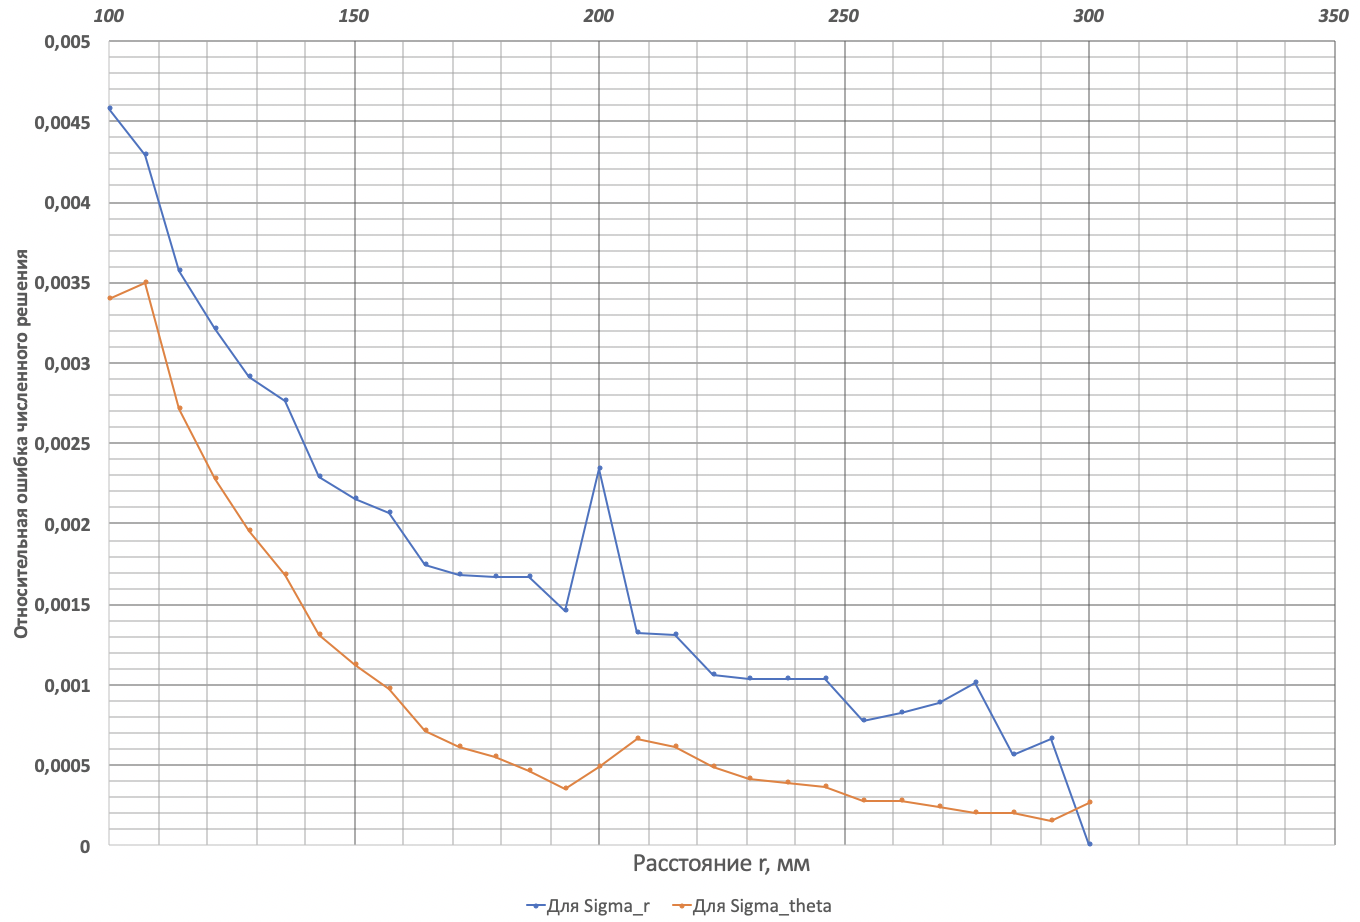
\includegraphics[scale=0.5]{img/error_Stress.png}\\
  \caption{Зависимость относительной ошибки численного решения для $\sigma_{11}$ и $\sigma_{22}$ от $r$.}
  \label{fig_18}
\end{figure}

\begin{figure}[H]
  \centering
  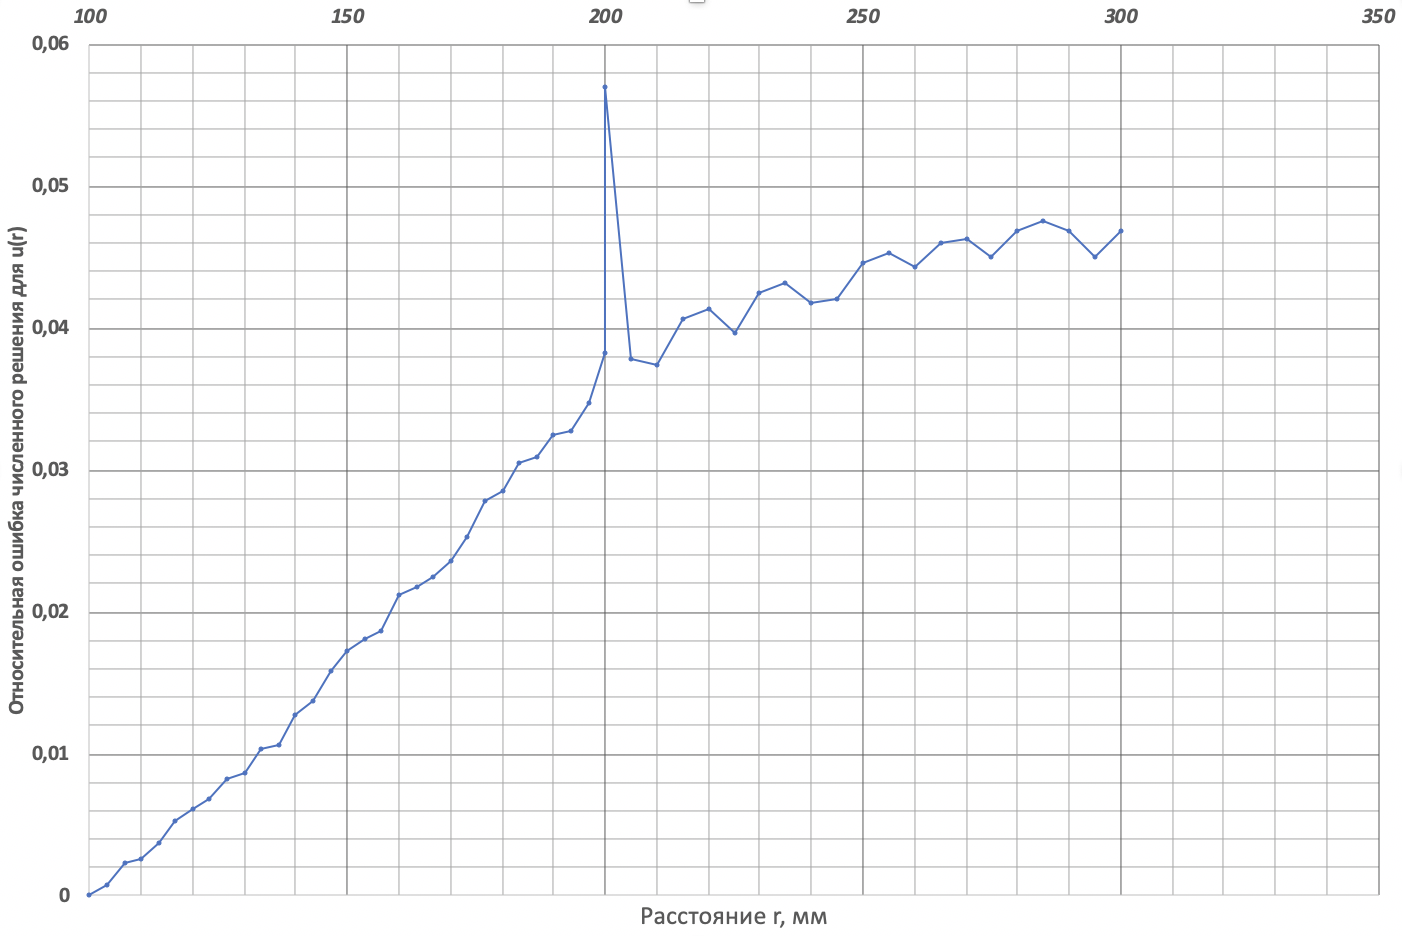
\includegraphics[scale=0.5]{img/error_u.png}\\
  \caption{Зависимость относительной ошибки численного решения $u_1$ от $r$.}
  \label{fig_19}
\end{figure}

\newpage

\Large
\section{Выводы}

\normalsize
В рамках линейной теории упругости получено аналитическое решение для задачи о напряжённо-деформированном состоянии составной толстостенной сферы, внутренняя и внешняя части которой выполнены из двух разных упругих материалов. Построены графики напряжений и перемещений при заданных параметрах материалов внешней и внутренней частей сферы.

Средствами конечно-элементного пакета ANSYS построены распределения напряжений и перемещений по сфере. Аналитические результаты были подтверждены расчётами в КЭМ-пакете ANSYS. Относительная ошибка численных решений не превышает $6\%$.

Полученное в рамках линейной теории упругости максимальное растягивающее напряжение стального слоя возникает на внутренней поверхности сферы и примерно равно 1750 МПа, что больше предела текучести (240 МПа) и предела прочности (820 МПа) стали.
Максимальное растягивающее напряжение медного слоя возникает на границе двух слоёв и примерно совпадает с пределом прочности меди (210 МПа). Следовательно, при заданных граничных условиях сфера разрушится.

Максимальная разница в аналитическом и КЭМ решениях для напряжений достигается при $r=0$, так как в этой области производная аналитического решения максимальна, а дискретизация величины в области, где она меняется быстро, ведёт к большей ошибке, чем дискретизация в области, где величина меняется медленно.
Максимальная разница в аналитическом и КЭМ решениях для перемещений достигается на границе слоёв, так как дискретизация области с резко меняющимися параметрами (модулем Юнга, коэффициентом Пуассона) ведёт к большей ошибке, и на внешней границе, так как она наиболее удалена от внутренней границы, на которую наложено условие на перемещение.
\end{document}
